% normal report style
\documentclass[10pt, a4paper]{report}

% thesis details
% ---------------------------------------------------------------------------
\newcommand{\thesisauthor}{Marcus Kossatz}
\newcommand{\titleFirst}  {Visualizing and Editing the}
\newcommand{\titleSecond} {Evolution of Countries in Time and Space}
\newcommand{\submissionDate}{6. June 2016}

\newcommand{\hg}{\textsc{HistoGlobe}}
% ---------------------------------------------------------------------------

%\*** INCLUDING PACKAGES ***\
\usepackage[utf8]{inputenc}     % encoding in UTF-8
\usepackage{lmodern}            % makes pretty font
\usepackage{amsmath}            % math mode with $ $
\usepackage{amssymb}            % several math symbols
\usepackage{textgreek}          % for Greek letters
\usepackage{cite}               % numerical citation
\usepackage{url}                % url mode for bibtex
\usepackage{graphicx}           % includegraphics
\usepackage{moreverb}           % for verbatimtab
\usepackage{fancyhdr}           % customise the page header
\usepackage{hyperref}           % cliackable toc
\usepackage{titletoc}           % manipulate toc
\usepackage{array}              % for removing vertical space of lists inside tabulars
\usepackage{supertabular}       % for tabular with page break
\usepackage{wrapfig}            % for floating text around images
\usepackage{geometry}           % set page margins manually
\usepackage{float}              % for positioning options for containers h!
\usepackage{pdfpages}           % include foreign pdf files
\usepackage{caption}            % to center captions figures
\usepackage[super]{nth}         % for 1st, 2nd, 3rd, ...
\usepackage{textcomp}           % gets rid of gensymb (v) package warning
\usepackage{gensymb}            % for ° symbol
\usepackage{alltt}              % allows symbols in something like verbatim
\usepackage{subcaption}         % allows multiple graphics per figure
\usepackage{booktabs}           % for fancy tables
\usepackage{multirow}           % for merging cells on multiple rows
\usepackage{paralist}           % for compactenum
\usepackage{adjustbox}          % for raisebox (vertically centering graphics in table)
\usepackage{pbox}               % for pbox (line break inside table cell)
\usepackage{scrextend}          % for addmargin (left indent of environment)
\usepackage{listings}           % for nice code syntax highlighting
\usepackage{longtable}          % for tables across multiple pages
\usepackage{rotating}           % for sidewaysfigure (90° rotated overviewimage)


%\*** HYPHENATION RULES ***\
\hyphenation{HistoGlobe} % no hypthenation!


%\*** FORMAT & STYLE ***\

% page margins
%\geometry{a4paper, top=25mm, left=30mm, right=30mm, bottom=30mm, headsep=10mm, footskip=12mm}

% set Helvetica (like Arial) as standard font for the document
\renewcommand{\familydefault}{\sfdefault}

% line spacing
\linespread{1.2}

% distance between footnotes and text
\setlength{\skip\footins}{20pt}

% set space to new paragraph, but no indent
\setlength{\fboxsep}{0pt}
\parskip 11pt plus 1pt minus 1pt
\parindent 0pt

% header-left: section name, header-right: nothing, bottom-center: page numbers
%\setlength{\headheight}{15.2pt} % latex hack that prevents error message
%\pagestyle{fancy}
%\rhead{\HG}

% make quotes italic
\newenvironment{quoteit}
{\begin{quote}\itshape}
{\end{quote}}


%\*** CODE SYNTAX HIGHLIGHTING ***\

% use a tt (monospace) font with a bold variant
\renewcommand{\ttdefault}{pcr}

% define pseudocode language
\lstdefinelanguage{pseudocode}
{
  % list of keywords
  morekeywords={             % define keywords
    FUNCTION,
    NEW,
    IF,
    ELSE,
    IS,
    ISNT,
    WHILE,
    FOREACH,
    IN,
    RETURN
  },
  sensitive=false,            % keywords are not case-sensitive
  morecomment=[l]{\#},        % l is for line comment
  morestring=[b]"             % defines that strings are enclosed in double quotes
}
% set style for pseudocode language
\lstset{
  language=     pseudocode,           % define the style for pseudocode
  frame=        single,               % frame around the code
  rulecolor=    \color{lightgray},    % color of frame
  numbers=      left,                 % position of line numbers
  numberstyle=  \tiny,                % font size of line numbers
  basicstyle=   \scriptsize\ttfamily, % initial font family and size
  captionpos=   b,                    % caption-position: bottom
  % set keywords and their style
  keywordstyle= \color{gray}\bfseries,
  % defines comments and their style
  commentstyle=\color{gray},
  comment=[l]{//}
}


%\*** NUMBERING AND TOC ***\

% counter for assumptions
\newcounter{assicounter}

% numbering of subsubsections
\setcounter{secnumdepth}{3}

% include chapter -> sections -> subsections in toc
\setcounter{tocdepth}{2}

% configure toc               left indent          space up/down      font                 position of numbers    filling until page number
\titlecontents{chapter}       [3.2em]  {\addvspace{+0.2em}\large\bfseries} {\contentslabel{2.2em}} {} {\hfill               \contentspage}
\titlecontents{section}       [6.7em]  {\addvspace{-0.6em}\large}          {\contentslabel{2.95em}}{} {\titlerule*[0.6pc]{.}\contentspage}
\titlecontents{subsection}    [10.6em] {\addvspace{-0.8em}\normalsize}     {\contentslabel{3.8em}} {} {\titlerule*[0.6pc]{.}\contentspage}
% \titlecontents{subsubsection} [14.5em] {\addvspace{-1.0em}\normalsize}     {\contentslabel{3.8em}} {} {\titlerule*[0.6pc]{.}\contentspage}

% configure clicking on toc
\hypersetup{
  colorlinks,
  citecolor=black,
  filecolor=black,
  linkcolor=black,
  urlcolor=black
}

% some weird hack to get rid of the vertical space in lists inside tabulars
\makeatletter
\newcommand*{\compress}{\@minipagetrue}
\makeatother

% allow for centering an table column width {cx}
\newcolumntype{x}[1]{>{\centering\arraybackslash\hspace{0pt}}p{#1}}

% use bullets for itemize
\renewcommand{\labelitemi}{$\bullet$}

% allow 90° rotated column titles in tabular
% usage: \rot{title column}
\newcommand*\rot{\rotatebox{90}}

% meta information
\title{\titleFirst \\ \titleSecond}
\author{\thesisauthor}
\date{\submissionDate}


%%%%%%%%%%%%%%%%%%%%%%%%%%%%%%%%%%%%%%%%%%%%%%%%%%%%%%%%%%%%%%%%%%%%%%%%%%%%%%%%

\begin{document}

%\* TITLE PAGE *\

%!TEX root = ../masters_thesis.tex

\begin{titlepage}

Bauhaus-Universität Weimar \\
Faculty of Media \\
Degree Programme Computer Science and Media \\ [2.0cm]

\begin{center}

{\huge \titleFirst} \\[0.5cm]
{\huge \titleSecond} \\[3.5cm]
\end{center}

{\LARGE Master's Thesis} \\[1.0cm]

Marcus Kossatz \hfill Matriculation Number 90487 \\
b. 21.08.1989 in Spremberg, Germany \\

1. First Referee: Univ.-Prof. Dr.-Ing. habil. Volker Rodehorst \\
2. Second Referee: Prof. Dr. rer. nat. Sven Bertel \\

\vfill
Submission date: \submissionDate

\end{titlepage}


%\* LISTINGS *\

\tableofcontents

% reduce font size of lists
\begin{footnotesize}
  \listoffigures
  \listoftables
\end{footnotesize}

%\* META *\

%!TEX root = ../masters_thesis.tex

\section*{Selbstständigkeitserklärung}

\vspace{1em}

Hiermit versichere ich, dass ich die vorliegende Masterarbeit selbstständig und nur unter Zuhilfenahme der angegebenen direkten und indirekten Quellen erstellt habe. Diese Arbeit wurde in gleicher oder ähnlicher Form noch bei keinem anderen Prüfer als Prüfungsleistunf eingereicht und ist noch nicht veröffentlich.

\vspace{3em}

\section*{Statement of Authorship}

\vspace{1em}

Hereby I declare that I completed this Master's Thesis on my own and that information which has been directly or indirectly taken from other sources has been noted as such. Neither this, nor a similar work, has been published or presented to an examination committee.

\vspace{5em}

\hfill \rule{120px}{0.5px} \\
Weimar, \submissionDate \hfill Marcus Kossatz

\newpage
%!TEX root = ../masters_thesis.tex

\section*{Acknowledgements} % (fold)
\label{sec:acknowledgements}

Helau

% section acknowledgements (end)



%\* CONTENT *\

%!TEX root = ../masters_thesis.tex

% basic idea: given initial state $t_0$, consecutively insert Hivent Operations changing this state
% current state: accumulate all changes

\chapter{Introduction} % (fold)
\label{cha:introduction}
\begin{large}
\begin{quoteit}
  Imagine there's no countries \\
  It isn't hard to do \\
  Nothing to kill or die for \\
  And no religion too \\
  Imagine all the people \\
  Living life in peace
\end{quoteit}
\end{large}
\hfill \textit{-- John Lennon, \emph{Imagine} (1971)}

The song of John Lennon is an anthem for peace on Earth, for brotherhood of people, for the end of materialism -- but also for the end of countries. He connects the concept of a country to nationalism that encourages people to fight and die for. John Lennon wrote the song in the 1970s, in the midst of the Cold War between the capitalistic and the socialistic bloc, only 30 years after World War II and 50 years after World War I. Especially in Europe this time point would have probably not been described as ``peaceful''. And not just John Lennon connected this lack of peace with the existance of national states divided by artificial borders.

Now, another 45 years later, the situation in Europe looks much different: Most countries are united in a confederation of a largly shared economy. While there are still countries with clearly defined borders, they are mostly of legal nature, but citizens of the European Union can travel freely within large parts of Europe. This concept is celebrated as a major achievement, but it is mostly forgotten that the concept of nations with solid borders has not been there 200 years ago. While travelling back then was probably not as pleasent as it is today, Goethe at least did not need a passport when he travelled to Italy and back to Weimar. He also did not travel not from country ``Germany'' via ``Austria'' to ``Italy'', but he rather crossed several duchies and principalities that do not exist anymore.

% ==============================================================================
\section{Motivation} % (fold)
\label{sec:motivation}

What we might call ``our country'' today has changed a lot in the past. Hardly any of the current 193 member states of the United Nations are in their same border as 100 years ago. The countries have evolved in time and space. Would it not be nice to see this development? Would it not be nice to have a map that shows the state of the world at any point in history? With that map we can see how our country looked like 100 years ago. 200 years ago. 1000 years ago. We could see how settlements became cities and principalities became national states. While there are many historical sources describing one point in history, may it be governmental bills, historical maps or diary entries of kings, there is no such thing as a comprehensive historical world atlas that lets you travel back in time and space and explore \emph{when} our country changed, \emph{where} it changed -- and most importantly \emph{why}? This thesis is all about that: How can the historical development of countries be shown, for the benefit of a better understanding of how we became what we are today.

This is a very complicated undertaking, given that countries have changed frequently. But there are severe conceptual problems: How do we know how a country has looked like in 1600? And if we find an historical map of this time, can we trust it? How certain can we be that the countries and their borders are true? The next problem is that the history of countries can also be contradictory. There is not always \emph{one story} which is supported by all sides. There are contested territories, even today, from which it is not clear who they belong to. There are ``places'', even today, which are not clearly a ``country'' because some might disagree. There is a whole lot of uncertainty and diagreement in the history of countries that this thesis deals with.

Finally, the state of the world can not be visualized at any point in history just like this -- because there is no freely available dataset. It is not just a visualization problem, it is a data problem. And to go even further: It is a data model problem because it is not even straightforward to say what kind of information is actually necessary to show the history of countries. And if we found a data model and got some data, we do not want to write it into a database table. The third goal for this thesis is to develop a well-designed user interface to edit the history of countries directly on the map.

% section motivation (end)

% ==============================================================================
\section{Problem Domain} % (fold)
\label{sec:problem_domain}

\begin{quoteit}
  All human actions takes and makes place. \\
  The past is the set of places made by human action. \\
  History is a map of these places. \\
  The past thus exists not in time but in space.
\end{quoteit}
\hfill -- Philip J. Ethington in \cite[précis]{citeTakeMakePlace}

\emph{Time} and \emph{space} are everywhere. They are highly related to our lives and the objects we perceive. The temporal perception of the world is driven by events, may they be personal life events like a wedding or world events like the Fall of the Berlin Wall. While a point in time can be described by a date and a time stamp, it is not always easy to scale and grasp. This is mainly because some temporal developments happen suddenly, like a natural disaster, and some happen very slowly throughout years, decades or even centuries, like climate change. Time is not tangible. For space, the situation is different, because it can be perceived as physically existing: A place is just there, we can go there and see it. Each point on this planet can be exactly described by a pair of geographic coordinates.

The combination of both concepts in one information system would allow to say how something has developed in time and space. \emph{Geographic Information Systems} (GIS) allow to manage and visualize data with a spatial relation to the Earth, mostly on a map. Most GIS answer two basic questions about an object: \emph{Where} it is in relative or absolute location and \emph{what} it is -- an object with certain properties. As an example, a country can be expressed by a set of borders consisting of border points in geographic coordinates and by a name. However, most of the current GIS are limited to the spatial dimension. They can not answer to the question \emph{when} a country was found or how its borders have developed in the previous fifty years. For that purpose \textbf{\emph{Historical Geographic Information Systems}} (HGIS) were developed. They extend general GIS with the dimension of time.

There are several \emph{spatio-temporal data models} that deal with the temporal development of spatial objects. The straightforward approach immediately derives from the the concept of historical maps: At certain time points a \emph{snapshot} is taken: a map showing the current state at this point in time. Snapshots can immediately answer the question how the the world has looked like at this date. However, they fail to answer the next question: What has changed since last time, when and why? Given two historical maps of Germany, one at 1871 after the formation of the German Empire and one 1919 after the Treaty of Versailles -- how did it look like at the beginning of World War I in 1914?

\begin{figure}[H]
  \vspace{1em}
  \centering
  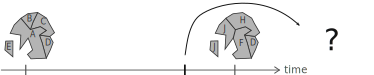
\includegraphics[width=0.8\textwidth]{graphics/introduction/snapshot_approach}
  \caption{The snapshot approach for modelling time and space}
  \label{fig:snapshot_approach}
\end{figure}

As it is seen in figure \ref{fig:snapshot_approach}, this is impossible to say, because there is no information about an arbitrary time point between two snapshots. Also, if the map only shows Germany and its neighboring countries, what about Russia, Sub-Saharan Africa or South East Asia? For an interactive historical world atlas, the snapshot approach is neither suitable nor feasible, because it requires a whole new world map every time some country changes on Earth.

The key problem is that snapshots can not say what has changed, because they do not store changes. This is the approach of another class of spatio-temporal data models: \emph{Event-based} models. They store two things: one reference snapshot and a set of events that happen at a certain time point and trigger changes on the map relative to the last event.

\begin{figure}[H]
  \vspace{1em}
  \centering
  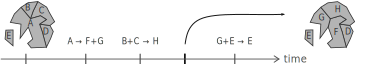
\includegraphics[width=0.8\textwidth]{graphics/introduction/event_based_approach}
  \caption{The event-based approach for modelling time and space}
  \label{fig:event_based_approach}
\end{figure}

Figure \ref{fig:event_based_approach} shows an example of an event-based approach. There are three changes that consecutively happen to the snapshot on the left. The question how the world looked like at an arbitrary point in time can be answered like this: It is the state of the reference map and all the changes of all events since that time point accumulated. In the case of figure \ref{fig:event_based_approach}, country $A$ split up into $F$ and $G$ and $B$ and $C$ have unified to $H$. This approach is suitable for modelling a countries history, because each change to the state of a country was introduced by some historical event, may it be a declaration or a peace treaty.

% ------------------------------------------------------------------------------
\paragraph{Research Questions} % (fold)
\label{par:research_questions}

The goal of this thesis is to lay a theoretical foundation for an Historical Geographic Information System that deals with the development of countries in time and space. The domain is limited to countries, their names and their borders and historical events that change them. In addition, the model is to be developed in HistoGlobe, open-source Web-based application that aims to visualize the course of history. It should provide a well-designed user interface for editing historical data about countries allowing the user to directly manipulate the countries on the map.

For that matter there are three research questions to be answered throughout the thesis:

\begin{enumerate}
  \item What type of historical changes can happen in the development of countries in time and space?
  \item How can these changes be
  \begin{enumerate}
    \item modeled in an information system?
    \item edited by humans in a user interface?
  \end{enumerate}
  \item How can the model handle uncertainty and disagreement in history?
\end{enumerate}

% paragraph research_questions (end)

% ==============================================================================
\newpage
\section{Overview} % (fold)
\label{sec:overview}

The remaining part of this Master's thesis is structured in four chapters. The second chapter introduces the basic concepts of the problem domain: First of all the suprisingly difficult concept of a \emph{country} is introduced in section \ref{sec:countries}. Afterwards the term \emph{Historical Geographic Information Systems} is clarified in section \ref{sec:historical_geographic_information_systems}), followed by state of the art of \emph{spatio-temporal data models} (\ref{sec:spatio_temporal_data_models}). The last section \ref{sec:histoglobe} presents \emph{HistoGlobe}, the application that the work of this thesis is developed in.

Chapter 3 is the main part of this thesis. It describes the Human Centered Design process to answer the first two research questions: The \emph{Hivent Model} in section \ref{sec:hivent_model} introduces a set of five \emph{Hivent Operations} that can model all possible changes to the development of countries in time and space. The next section \ref{sec:editing_hivent_data} presents approaches to edit data in the Hivent Model using \emph{Edit Operations}, a different set of operations that is well-understood by humans. The iterative design process of the user interface is illustrated in section \ref{sec:user_interface_design_process}. The chapter closes in \ref{sec:implementation} with an insight into the implementation of the data model and the user interface in the HistoGlobe application.

The fourth chapter tackles the last research question: How to deal with uncertain historical data? The model and the implementation of chapter 2 are evaluated in section \ref{sec:evaluation}. From the identified shortcomings the thesis developed approaches to handle some aspects of uncertainty regarding the historical development of countries. The designed extensions are presented in section \ref{sec:modelling_uncertainty}.

In the last chapter the work of the thesis is summarized.

% TODO: finish

% section overview (end)

% ==============================================================================

% chapter introduction (end)
%!TEX root = ../masters_thesis.tex

% TODO: all examples as close as possible to the actual domain

\chapter{Basics} % (fold)
\label{cha:basics}

This chapter will lay the theoretical foundation of this Master's Thesis and will embed it into the context of current research. The title of this work is:

\vspace{-1em}
\begin{center}
\textbf{\titleFirst \\ \titleSecond}
\end{center}

It includes the domain (\emph{history of countries}) and the system to acquire, model, manage and visualize data of the domain: \emph{Historical Geographic Information Systems} (HGIS).

The first section of this chapter will define HGIS and related terms. Afterwards, concepts to model time and space in an information system are introduced. Data sources suitable for input into an HGIS are listed in the next section, followed by techniques to manage and analyse the data.
%A special focus lies on concepts to visualize spatial and temporal data, explained in the next section. The chapter closes with possible HGIS applications and introduces the tool that is used in this thesis: HistoGlobe.

extension of Hivent model to actors

% TODO: country
% TODO: enclaves and exclaves


% ==============================================================================
\section{Historical Geographic Information Systems} % (fold)
\label{sec:historical_geographic_information_systems}

\begin{quoteit}
  ``All human actions takes and makes place. The past is the set of places made by human action. History is a map of these places. The past thus exists not in time but in space.''
\end{quoteit}
\hfill -- Philip J. Ethington in \cite[précis]{citeTakeMakePlace}

An Historical Geographic Information System helps to answer research questions about how geographical phenomena have developed over time. To understand how it works, it is important to understand the four parts of the word: The research fields \emph{history} and \emph{geography} and the concepts of \emph{information} an \emph{systems}.


% ------------------------------------------------------------------------------
\subsection{History} % (fold)
\label{sub:history}

History is ``an ideal field for thinking long and hard about important questions''
\cite{ahaFiveCs}.
The Greek word \emph{\textIota\textsigma\texttau\textomikron\textrho\textiota\textalpha / historia}, meaning ``finding out, learning through research, narration of what is learned'', is the origin
\footnote{
  \emph{History},
  Dictionary.com, based on Random House Dictionary, 2015,
  URL: \url{http://dictionary.reference.com/browse/history},
  last access: 23.10.2015
}
and it signifies the two main modern usage forms of the term: To research about and learning something and to tell a story. There are many different definitions of the word \emph{history}
\footnote{
  \emph{History},
  Merriam Webster -- an Encyclopædia Britannica Company,
  URL: \url{http://www.merriam-webster.com/dictionary/history},
  last access: 23.10.2015
}.
The main goal of history is to study processes in the past to understand the situation in the present and make reasonable decisions for the future. The American Historical Association has developed the ``five C`s of historical thinking [that] together describe the shared foundations of [the] discipline''\cite{ahaFiveCs}:

\vspace{-1em}
\begin{description} % manipulation of indentation
  \item[Change over time]
  The lives of people, their languages and their cultures are continuously changing. Describing these historical changes, triggered by historical events happed in the past, is a major goal of history. Snapshots in the form of historical maps or historical photography are used to tackle this task.
  %TODO: refer to this in later sections
  \item[Context]
  is an important element of historical thinking. The goal is to travel back in time to the moment of the event and recreate the world based on primary sources. The understanding of the historical context is crucial for the understanding of the event.
  \item[Causality]
  The overall goal of each science is to answer the \emph{why}-question concerning an event or a process. For historians that means to reasonably explain an historical event or process based on evidence. The problem is that history is not a science that can alter experimental conditions to extract new information, in a way that e.g. experiments in physics work. Historians have to focus on the interpretation of primary sources, which inherently yields multiple explanations for a single event.
  \item[Contingency]
  is a derived aspect from this problem. Each event has a whole network of prior conditions, because the world is highly interconnected. A slight change in one prior condition could have led to a completely different outcome of the event and a different state of the world.
  \item[Complexity]
  The intrinsic human need for order conflicts with the complexity of history and their events and processes, because of its contingency. It is questionable if all details about events in the world are scientifically explainable.
  %This problem is comparable to the Heisenberg problem in physics: Whereas on the macro-level e.g. physical movements are a direct cause of a set of preconditions (speed, fraction, wind, weight, ...) and are therefore predictable, the smallest of all particles are not traceable, their movements are not predictable and therefore their processes not explainable.
\end{description}

Historical research is conducted by studying and interpreting primary sources, such as written documents, verbal texts, speeches, photographs, audio, video or historical maps. This signifies that most historical research is qualitative. The main organization principle in history is periodization: classifying events and processes to describe broader long-term changes and to explain complex phenomena
\cite[pp.4-7]{knowles2008placing}.
A special focus in this thesis is laid on historical maps as primary source to extract spatial information.

% subsection history (end)

% ------------------------------------------------------------------------------
\subsection{Geography} % (fold)
\label{sub:geography}


The term ``geography'' comes from Greek ~\emph{\textgamma\textepsilon\textomega\textgamma\textrho\textalpha\textphi\textiota\textalpha / geographia}~, literally ``describing the earth.''
\footnote{
  \emph{Geography},
  Dictionary.com, based on Random House Dictionary, 2015,
  URL: \url{http://dictionary.reference.com/browse/geography},
  last access: 23.10.2015
}
It is a science that studies the interplay between the landscapes and environments of the Earth (\emph{physical geography}) on the one hand and the people, their cultures, societies and economies (\emph{human geography}) on the other. That means geography is an interdisciplinary field between natural and social sciences
\cite{rgsGeography}.

Geographical research aims to understand where things are found, why they are there and how they developed over time.
% In regional geography, another subbranch, also the causes of social or environmental differences between cultures and landscapes want to be found.
It focuses on the interconnectivity between elements of physical and human geography, which gets expressed in Tobler's First Law of Geography: ``Everything is related to everything else, but near things are more related than distant things.''
\footnote{
  ``A computer movie simulating urban growth in the Detroit region'',
  Waldo Tobler, 1970
  Economic Geography, 46(2): 234-240.
}

Geographers use different technology and techniques to analyze geographic processes and to answer their research questions. The oldest and most important among those are maps. A map is a graphical expression of something that is not tangible: a part of the real world. A map shows the physical, environmental, political, economical or social properties of the Earth in order for the user of the map to get the most relevant information for his task, may it be orientation, learning or teaching. The ``art and science of making maps'' is the field of \emph{cartography}
\footnote{
  \emph{History of maps and cartography},
  James S. Aber,
  URL: \url{http://academic.emporia.edu/aberjame/map/h_map/h_map.htm},
  last access: 24.10.2015
}. Since maps visualize a model, they have a natural constraint: ``No map can perfectly replicate the real world, since it inevitably generalizes, abstracts and approximates the complexity of the reality''
\cite[p. 181]{knowles2008placing}.

% TODO:                 had? had? has had? is having?
% The scientific background of GIS is \emph{geographic information science} (GISci) that studies patterns in natural and human development, e.g. erosion of valleys, literacy rate, natural hazards and deals with approaches and techniques to manage, analyze and visualize this information
% \cite{ngGeography}.


\paragraph{Comparison between geography and history} % (fold)
\label{par:comparison_of_geography_and_history}

Both research fields utilize maps for answering their research questions, which is the main commonality for the work of this thesis. However, the nature of both fields are also very different, illustrated in table \ref{tab:history_vs_geography}.

\begin{table}[ht]
\begin{center}
\begin{tabular}{p{0px} r c l p{0px}}
    \toprule
    & geography
    & difference
    & history
    & \\
    \midrule
    & where
    & dimension
    & when
    & \\

    & exact, statistical
    & character
    & complex, fuzzy
    & \\

    & mainly quantitative
    & research
    & qualitative
    & \\

    & spatial proximity of conditions
    & causal explanation
    & temporal sequence of events
    & \\

    & spatial differentiation
    & explanation
    & temporal differentiation
    & \\

    & clustering
    & ordering
    & periodization
    & \\

    & mostly visual (maps)
    & expression
    & mostly verbal (texts)
    & \\

    & high (GIS)
    & digitalization potential
    & low (digital humanities)
    & \\
    \bottomrule
\end{tabular}
\caption{differences between history and geography \cite[pp. 2-4]{knowles2008placing}}
\label{tab:history_vs_geography}
\end{center}
\end{table}


Whereas geography answers the questions \emph{where?}, history focuses on \emph{when?} -- but the ultimate goal for both sciences is to answer the question \emph{why?}

% paragraph comparison_of_geography_and_history (end)


% subsection geography (end)

% ------------------------------------------------------------------------------
\subsection{Information} % (fold)
\label{sub:information}

The terms ``signs'', ``data'', ``information'' and ``knowledge'' are sometimes used interchangeably and there is no coherent definition for any of them. However, all describe different concepts. This explanation seen in figure \ref{fig:information} is based on the work of \cite{datinfwis}.

\begin{figure}[ht]
  \vspace{1em}
  \begin{center}
    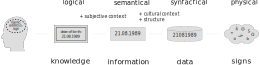
\includegraphics[width=0.9\textwidth]{graphics/basics/information}
  \end{center}
  \caption{signs, data, information and knowledge}
  \label{fig:information}
\end{figure}

A \emph{sign} is the physical representation of something in the real world. Since the real world is continuous, literally anything can be seen as a sign, so there are uncountably infinitely many different signs. \emph{Data} is a subset of all possible signs and represents the syntactical level of what an information system deals with. Data itself does not have any meaning, but as soon as it is organized, it becomes \emph{information}. However, information is sensitive to its cultural context. The string ~\texttt{14.07.1789}~ is useful and understandable for people in countries that use the date format \texttt{DD.MM.YYYY}. However, for people in Belize and the USA, that use the format \texttt{MM.DD.YYY}, this might just be a random string of numbers without any meaning, and therefore no information -- although it is the same data. If information is visualized to and understood by a human and it can be integrated into his or her larger subjective context, it is \emph{knowledge} \cite{nake}. The goal of a visualization is to present as much information as possible in a way that it can be transformed into knowledge by the viewer.

% subsection information (end)

% ------------------------------------------------------------------------------
\subsection{System} % (fold)
\label{sub:system}

A \emph{system} is an organized structure containing \emph{elements} or \emph{components} that are directly or indirectly \emph{related} to and \emph{interconnected} with each other. The elements and their relations form the whole of the structure. The surrounding of the system is its \emph{environment}. There is an \emph{internal state} at any point of the system's existence. This state only changes when it gets influenced by stimuli of its environment. \emph{Emergent properties} characterize a system. They are independent from properties of the element of the system, e.g. water is liquid at room temperature, but the elements it consists of, hydrogen and oxygen, are a gas. Each system is both part of a larger system and can be decomposed into subsystems. Therefore, systems form a hierarchy.

A system has defined spatial and temporal boundaries. There are two types: \emph{open systems} allow exchange of energy or information with their environment, whereas idealized \emph{close systems} naturally do not interact with and are not influenced by its environment. Based on the black box principle the inner working of a closed system can not be seen from the outside
\cite{system}.

% subsection system (end)

% ------------------------------------------------------------------------------
\subsection{Motivation} % (fold)
\label{sub:motivation}

An \emph{information system} (IS) is an application that is dealing with the acquisition, management, analysis and presentation of information. It is the unity of all its components and their interaction with each other
\cite{informationSystem}.
If the majority of the information in a system has a spatial relation to the Earth, its surface, its lithosphere, atmosphere or the social or economical structure of its habitation, it is a \emph{geographic information system} (GIS). The data objects in the system are called \emph{geo-objects}
\cite{bolstad2008gis}.
If the information additionally has a temporal dimension, e.g. via time stamps or time spans, which enable to trace developments of geo-objects, it becomes an \emph{Historical Geographic Information System}
\cite{gregory2014toward}
or alternatively \emph{Spatio-Temporal Information Systems} (STIS)
\cite{pelekis04stdms}.

HGIS react on the spatial turn of history: the integration of geographic methods in historical research. It aims to discover the power of cartographic representation: ``The spatial turn in the humanities must [...] understand the role of space in human events''
\cite{bodenhamer2010spatial}.
At the same time, they are the product of the temporal run in GIS: the coexistence of space (where things are) and time (what has changed over time)
\cite[p. 45]{solana2014spatio}.
With HGIS it is possible to analyze how ``spatial patterns change over time in order to better understand large-scale Earth processes''
\cite{peuquet99}.
Since ``the world never stands still'', but ``the retention of information relating to past events [is] an important element of human representation of the world'', the dimension of time has to be integrated into a GIS
\cite{peuquet99}.

HGIS are rather recent tools and used mostly in \emph{Digital Humanities} as a digital tool to answer research questions in the traditional fields of humanities: ``situating history in its geographical context and using geographic information to illuminate the past''
\cite[p. 3]{knowles2008placing}.
Some interesting research questions that could be answered using HGIS could be:

\begin{compactitem}
  \item Did the European Union help to bring peace on the European continent?
  \hfill \emph{(political)}
  \item Is there a coherence between life expectancy and fertility rate?
  \hfill \emph{(social)}
  \item What is the effect of global warming on the melting of glaciers?
  \hfill \emph{(physical)}
  \item What was the effect of Bismarck's foreign policy on peace in Europe?
  \hfill \emph{(historical)}
\end{compactitem}

Or on a more abstract level: Where and When has something changed and why did it change?

% subsection motivation (end)

% ------------------------------------------------------------------------------
\subsection{Components} % (fold)
\label{sub:components}

Information systems in general are based on a data model --- HGIS in particular on a \emph{spatio-temporal data model}, introduced in section \ref{sec:spatio_temporal_data_models}. On top of that, there are different components. One way to classify them is using the four-component model:

\begin{enumerate}
  \item \textbf{Input}: Primary acquision of spatio-temporal data, i.e. historical events, historical and current countries and their territories.
  \item \textbf{Management}: Physical storage and logical management of the data in a spatio-temporal database, using a structure that fits the spatio-temporal data model.
  \item \textbf{Analysis}: Gaining spatio-temporal information by cleaning, transforming or combining the data in database.
  \item \textbf{Presentation}: Visualization of information on different displays, e.g. a map and a timeline, transforming information into spatio-temporal knowledge.
\end{enumerate}

% subsection components (end)

% ------------------------------------------------------------------------------
\subsection{Applications} % (fold)
\label{sub:applications}

``Today, operational temporal GIS does not exist''. This quote summarizes the state of the art in this field. The main reasons are ``the complexity of integrating space and time and the lack of standards''
\cite[p. 5]{raza12}.

However, there are numerous project that use HGIS for one specific research question. A large collection them can be found in \cite{knowles2008placing} and \cite{gregory2014toward}. A famous visualization combining time and space Napoleons Moscow Campaign by Charles Minard from 1869 (see figure \ref{fig:minard_napoleon}). The ``best statistical graphic ever drawn''
\footnote{
  \emph{The Visual Display of Quantitative Information} (p. 40),
  Edward R. Tufte,
  2001
}
shows the number of men in Napoleon’s 1812 Russian campaign army, their movements, as well as the temperature they encountered on the return path
\cite[pp. 188-191]{knowles2008placing}.

\begin{figure}[ht]
  \centering
  \includegraphics[width=0.8\textwidth]{graphics/basics/napoleon_march_moscow.png}
  \caption{Napoleons Moscow Campaign \protect\footnotemark}
  \label{fig:minard_napoleon}
\end{figure}

\footnotetext{
  \emph{Minard.png}
  Charles Minard, 1869,
  URL: \url{https://commons.wikimedia.org/wiki/File:Minard.png},
  last access: 03.11.2015,
}

The \emph{Great Britain Historical GIS Project} (GBHGIS)
\footnote{
  \textit{Great Britain Historical Geographical Information System (GBHGIS)},
  Ian Gregory \& Humphrey R. Southall, University of Portsmouth, since 1994,
  URL: \url{http://www.port.ac.uk/research/gbhgis/},
  last access: 02.11.2015
}
combines statistical data with territorial units of the United Kingdom, e.g. to analyze net migration in the districts in UK. The data is collected by the \emph{British Ordnance Survey}, who automatically detect spatial changes to the geography and land use of the United Kingdom using aerial photography
\footnote{
  \textit{British Ordnance Survey},
  URL: \url{https://www.ordnancesurvey.co.uk/education-research/research/automatic-change-detection.html},
  last access: 02.11.2015
}.

The \emph{National Historical Geographic Information System} (NHGIS)
\footnote{
  \textit{Welcome to NHGIS},
  Minnesota Population Center, University of Minnesota,
  since 2007,
  URL: \url{},
  last access: 02.11.2015
}
provides the digital boundaries of the United States of America and census data for each year since 1790.
% \cite{aerialInterpolation}
While the data in the system is extensive, the interface to analyze and use the data is very frustrating to use: A tutorial is necessary to go through the selection process. To download data, a user has to register, receive an email with a link to download a compressed file which has to be decompressed and then loaded into a GIS software to be visualized.

HGIS are not widely accepted in the humanities. One reason is the nature of the qualitative historical research: historic sources are subjective and biased, their content may be fuzzy and they are definitely incomplete. So the knowledge that can be extracted from a source bears the integral problem of \emph{uncertainty}. Information systems on the other hand have a logical architecture and, to be as precise and accurate as possible. Analysis is based on mathematical functions -- an information system is quantitative in its entire nature
\cite[p. 2]{knowles2008placing}.

% subsection applications (end)

% section historical_geographic_information_systems (end)


% ==============================================================================
\section{Time and Space} % (fold)
\label{sec:time_and_space}

This section will explain ways to separately represent time and space in an information system. It will first explain the geospatial data model used in traditional GIS and then introduce maps as the representation of spatial information. In the second part of the chapter, models to represent the temporal dimension are introduced.

% ------------------------------------------------------------------------------
\subsection{Model of Geographical Space} % (fold)
\label{sub:model_of_geographical_space}

HGIS need to unambiguously locate geo-objects on, underneath or close to the Earth's surface using \emph{geographic coordinates}. They express an object directly in the coordinate system of the Earth. To understand that, a model of the Earth has to be developed, the \emph{geodetic datum}, that needs to fit the real shape of the Earth as accurately as possible.

% - - - - - - - - - - - - - - - - - - - - - - - - - - - - - - - - - - - - - - -
\paragraph{The shape of the Earth} % (fold)
\label{par:the_shape_of_the_earth}

measured in the field of \emph{geodesy} is very complicated. In the Babylonian Empire ($\approx$ 2000-539 BC) the theory of the Earth being a flat disc surrounded by an infinite body of water
%(a theory still valid in some southern parts of the United States of America)
evolved. The Greek scientists Pythagoras and Aristotle (340 BC) rejected this theory and proved the earth to be a three-dimensional spherical object. It took almost 2000 years until Sir Isaac Newton (1687) reasoned that due to the centrifugal forces of the rotating Earth the shape has to be flattened at the poles and is therefore better described as an \emph{ellipsoid} with two radii: the polar radius ($r_p$) and the slightly larger equatorial radius ($r_e$)
\cite[pp. 69-77]{bolstad2008gis}.

However, the model disregards that the surface of the Earth is not flat but consists of deep oceanic trenches and high mountains. Therefore the gravitational field of the Earth is not homogeneous either: the actual \emph{mean sea level}, the reference surface for the height of objects varies from 106 meter below to 85 meter above the uniform sea level of the ellipsoid model. These discoveries in the \nth{20} century led to the complex \emph{geoid} model (see figure \ref{fig:geoid}). The latest and most accurate measurements for the shape of the Earth are the result of the GOCE satellite launched in March 2009
\cite{geoid, geoidESRI}.

\begin{figure}[H]
  \centering
  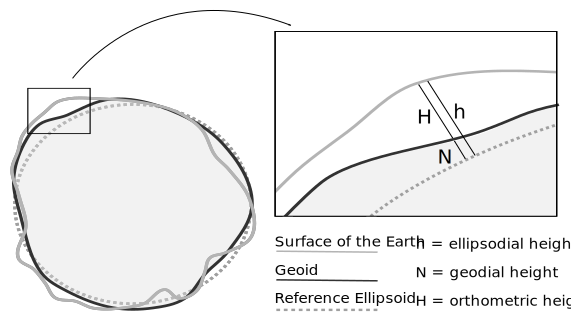
\includegraphics[width=0.72\textwidth]{graphics/basics/geoid}
  \caption{The geoid model, differences are exaggerated, \cite[Fig. 3-6, p. 75]{bolstad2008gis}}
  \label{fig:geoid}
\end{figure}

% paragraph the_shape_of_the_earth (end)

% - - - - - - - - - - - - - - - - - - - - - - - - - - - - - - - - - - - - - - -
\paragraph{Geographic coordinate system} % (fold)
\label{ssub:geographic_coordinate_system}

The basis for the geospatial data model is the reference ellipsoid. It is represented in a three-dimensional \emph{spherical coordinate system}. The \emph{North} and the \emph{South Pole} are defined as the two surface points closest to the Earth's center opposite to each other. The \emph{Equator} is the line equidistant to the two poles and dividing the world in a \emph{Northern} and \emph{Southern Hemisphere}. Additionally, the \emph{Prime Meridian} is defined as the line perpendicular to the Equator, running from the North to the South Pole. Since there are infinitely many lines like this, its definition is arbitrary, but by convention, the line running through Greenwich (London, United Kingdom) is used. Based on these two lines, each point in the spherical coordinate system can be unambiguously defined by
\cite[pp. 26-28]{bolstad2008gis}:

\begin{compactenum}
  \item The rotation angle along the Equator, defining its longitude: $\gamma = [-180\degree ~...~ +180\degree]$
  \item The rotation angle along the Prime Meridian, defining its latitude: $\phi = [-90\degree ~...~ +90\degree]$
  \item The distance to the origin: $r \in \mathbb{N}_0$
\end{compactenum}

\begin{figure}[ht]
  \vspace{1em}
  \centering
  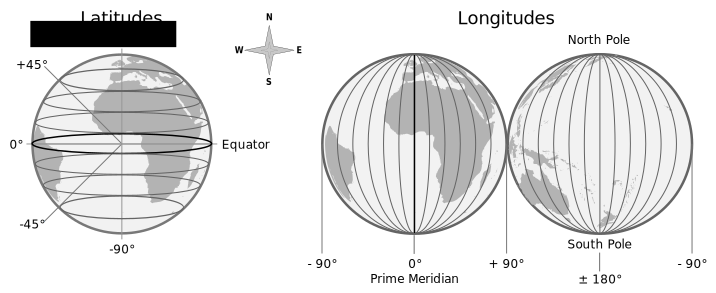
\includegraphics[width=0.8\textwidth]{graphics/basics/geo_coordinates}
  \caption{geographic coordinates using latitude and longitude}
  \label{fig:geo-coordinates}
\end{figure}

Lines of constant latitude are running horizontally and are called \emph{parallels}, lines of constant longitude are \emph{meridians} appearing in vertical direction. All parallels are circles with their center on the axis between the poles. No two parallels intersect. The longest parallel is the Equator (0\degree~latitude). All meridians have the same length. Geographic coordinates are usually recorded either in degree-minutes-second (\texttt{DMS}, e.g. \texttt{50\degree~58' 22''}) or in decimal degree (\texttt{DD}, e.g. \texttt{50.973}) notation
\cite[pp. 30, 79]{bolstad2008gis}.


% - - - - - - - - - - - - - - - - - - - - - - - - - - - - - - - - - - - - - - -
\paragraph{The Geodetic Datum} % (fold)
\label{par:geodetic_datum}

is the digital model of the analogue Earth. It consists of two parts: The approximation of the Earth's surface in a the Cartesian coordinate system with the origin in the Earth's center and a set of reference points used to accurately locate a point.

Geodetic datums can be very accurate in one region of the world, i.e. the model fits the real geoid very well, but inaccurate in another region. This is the main reason why there are a lot of different geodetic datums used in the world. The same coordinates in two different geodetic datums define two different points on Earth. In order to be accurate is essential to know the geodetic datum of the coordinates
\cite[p. 80]{bolstad2008gis}.
The \emph{World Geodetic System 1984 (WGS84)} is a model that found worldwide acceptance and is used in all major Web-based mapping services like \emph{OpenStreetMap} and in the GPS unit of major mobile devices.

% paragraph geodetic_datum (end)

% - - - - - - - - - - - - - - - - - - - - - - - - - - - - - - - - - - - - - - -
\paragraph{Raster and Vector Model} % (fold)
\label{ssub:raster_vs_vector_model}

The real world is infinite in detail, but storage in a computer system is finite. In order to model continuous geographical phenomena in an information system, a relevant subset of them has be sampled to create discrete spatial data. It can be represented in a raster or in a vector model.

\begin{figure}[H]
  \centering
  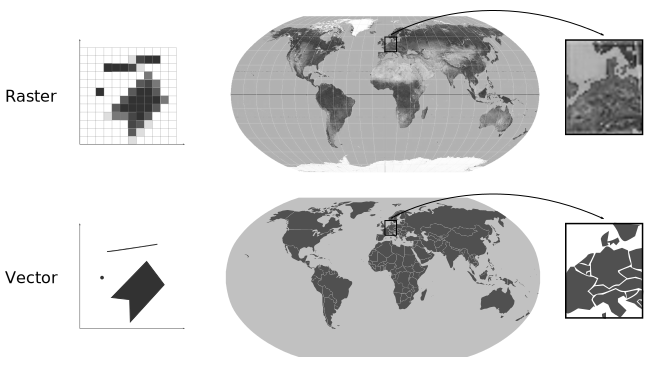
\includegraphics[width=0.75\textwidth]{graphics/basics/raster_vector}
  \caption{Comparison of the raster and the vector model}
  \label{fig:raster_vector}
\end{figure}

The \emph{raster model} contains a regular grid with a fixed \emph{cell dimension}. Each cell has a certain value, e.g. a color value.
The model is simple and allows straightforward rendering: only affine transformations have to be applied in order to project two raster map layers on top of each other. The main disadvantage of the raster model is its fixed resolution: it can not be scaled up without losing quality
\cite[pp.42-48]{bolstad2008gis}.
Raster graphics are used for map tiles by most map engines, e.g. in OpenStreetMap or the satellite image by NASA in Google Maps.
% \footnote{
%   \emph{Google Maps},
%   URL: \url{https://www.google.com/maps/@51.2090662,13.2328189,3563505m/data=!3m1!1e3},
%   Imagery \textcopyright2015 Landsat, Data SIO, NOAA, U.S. Navy, NGA, GEBCO, IBCAO, U.S. Geological Survey, Map data \textcopyright2015 Google, ORION-ME,
%   last access: 29.10.2015
% }.

In the two-dimensional \emph{vector model}, each object is a mathematically described geometric primitive. All of them can be expressed by three basic primitives (figure \ref{fig:geometric_primitives}):
\begin{enumerate}
  \item[0D] A \emph{point} is the fundamental object in vector geometry. It has no dimension, no size and is only defined by its position, specified in geographic coordinates. One point is independent from all others. Points can be used to represent the location of an event.
  \item[1D] A \emph{polyline} is constructed by an ordered set of points with at least one start and one end point. A border line can be expressed by a polyline.
  \item[2D] A \emph{polygon} is an ordered set of polylines creating a closed area. A polygon can be \emph{simple}, \emph{weakly simple} or \emph{complex} (see figure \ref{fig:polygon_properties}). The territory of a country without islands can be described by a polygon. If a country does have islands or overseas territories, a \emph{polypolygon} represents multiple separate polygons belonging to one logical entity.
\end{enumerate}

\begin{figure}[H]
  \centering
  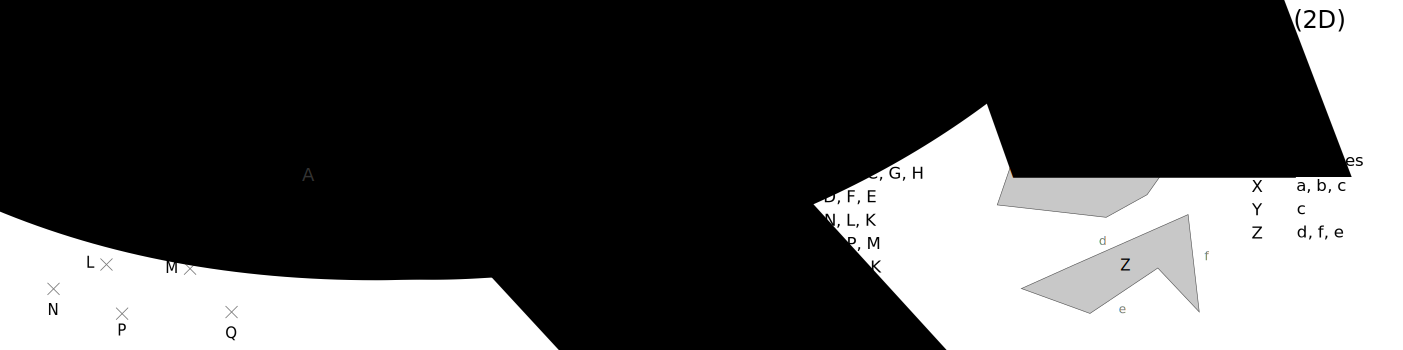
\includegraphics[width=0.8\textwidth]{graphics/basics/geometric_primitives}
  \caption{The basic geometric primitives point, polyline and polygon}
  \label{fig:geometric_primitives}
\end{figure}


\begin{figure}[H]
  \centering
  
\includegraphics[width=0.5\textwidth]{graphics/basics/polygon_properties}
  \caption{Different properties of polygons}
  \label{fig:polygon_properties}
\end{figure}

Scale-independence is one of the biggest advantages of a vector model. The data model is more compact in comparison to the raster model. On the other hand, the model can become very complex. Since vector data has to be rasterized to be shown on the screen, the computational effort increases with complexity \cite[pp.33-42]{bolstad2008gis}.
Vector models are suitable to represent phenomena that can easily to discretized, e.g. the boundaries of a country. Common file types for vector data with spatial reference are the open file format GeoJSON (\texttt{.geojson})
\footnote{
  \emph{GeoJSON},
  IETF GeoJSON Working Group,
  URL: \url{http://geojson.org/},
  last access: 30.10.2015
}
% and Scalable Vector Graphics (\texttt{.svg})
% \footnote{
%   \emph{W3C SVG Working Group},
%   IETF Geographic JSON Working Group,
%   URL: \url{http://www.w3.org/Graphics/SVG/},
%   last access: 30.10.2015
% }
or ESRI Shapefiles (\texttt{.shp})
\footnote{
  \emph{ESRI Shapefile Technical Description},
  ESRI White Paper, July 1998,
  URL: \url{http://www.esri.com/library/whitepapers/pdfs/shapefile.pdf},
  last access: 30.10.2015
}.

% paragraph raster_vs_vector_model (end)

% - - - - - - - - - - - - - - - - - - - - - - - - - - - - - - - - - - - - - - -
\paragraph{Geospatial Topology} % (fold)
\label{par:geospatial_topology}

\emph{Topology} is the study of position, how objects are spatially arranged and relatively positioned to each other. It does not include measures like distances or angles. Two objects are said to be topologically equivalent, if they can be deformed into each other, e.g. an ellipse can be stretched into a circle. A \emph{geospatial topological vector model} defines the relationship between geospatial objects, i.e. equals, disjoint, intersects, touches / neighbors, contains, covers, within, interior and boundary
\cite{clementiniTopology}.

The 2D vector model can be extended with a topology. The elements in this topological space are nodes (0D), edges (1D) and meshes (2D) and they correspond directly to the geometric primitives stated above. A topological vector model has strict connectivity (a ``clean'' geometry), if no two edges intersect without a node at their intersection point (planar), each interior edge has exactly two adjacent areas and each edge contains at least two nodes
\cite[pp.37-39]{bolstad2008gis}.

\begin{figure}[ht]
  \centering
  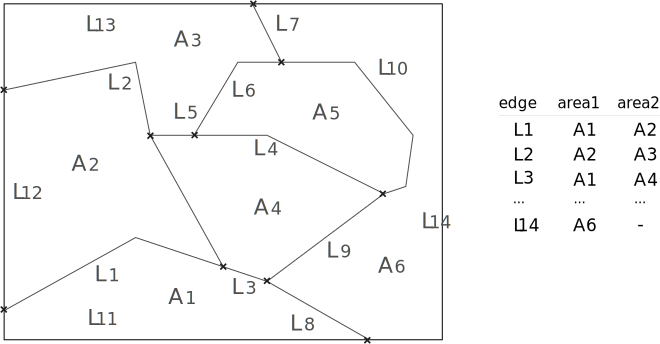
\includegraphics[width=0.55\textwidth]{graphics/basics/topological_vector_model}
  \caption{An example of a topological vector model and an adjacancy table}
  \label{fig:topological_vector_model}
\end{figure}

The topological vector model has a great asset: if an edge between two adjacent areas changes, the connectivity and adjacency does not change and therefore also the topology stays constant. The lookup for neighboring areas is very fast if the topology ensures strict connectivity: The neighbors of an area can be found in the adjacency table. Potentially problematic is the creation of a clean geometry: it can be cumbersome and require a lot of manual adjustment, for example ensuring strict connectivity by manually connecting nodes.

% paragraph geospatial_topology (end)

% subsection model_of_geographical_space (end)

% ------------------------------------------------------------------------------
\subsection{Presentation of Geographic Space} % (fold)
\label{sub:presentation_of_geographic_space}

The most common ways to present geographic space are two-dimensional \emph{maps} and three-dimensional \emph{globes}. The HGIS in this thesis will use a map to show the development of countries over time. A map is a discrete graphical expression of the geographical features of the continuous real world. The creation of a map is not just a scientific, but also a creative process: The form, function and interaction methods shall follow the purpose of the usage of the map.

A map is typically structured according to the \emph{layer} principle: Each layer is a transparent film showing one specific aspect, e.g. a physical layer showing coastlines, mountains or forests, a political layer showing international borders or a cultural layer showing cities or population densities. The layers are interchangeable, can be switched on and off and serve to serve a different visualization purpose. A \emph{legend} including the scale bar and north arrow shall explain all symbols used on the map and give orientation. In interactive web based systems, there should be \emph{menus} with different visualization options, e.g. panning and zooming on the map, switching map layers on and off or changing the color scheme of the map
\cite[pp. 159-166]{bolstad2008gis}.

\emph{Leaflet.js} is ``an open-source JavaScript library for mobile-friendly interactive maps''
\footnote{
  \textit{Leaflet - JavaScript library for interactive maps},
  URL: \url{http://leafletjs.com/},
  last access: 02.11.2015
}
that offers functionality to embed a map with a chosen projection in on the client-side of a web based information system, use own map tiles, symbols and markers on the map and tools for zooming and panning.

\paragraph{Map projections} % (fold)
\label{par:map_projections}

Since the Earth is three-dimensional, but the map on the computer screen only two-dimensional, the model of the Earth has to be projected onto the map. But as previously discussed in subsection \ref{par:the_shape_of_the_earth}, the Earth is an inhomogeneous spherical object with a curved surface whereas the map is flat
\cite[p.79]{bolstad2008gis}.
That is why some features of the Earth will be distorted on the map: An \emph{equivalent projection} preserves the area sizes of features on the map, whereas a \emph{conformal projection} preserves angles and the shapes of objects. Every map projection that is area-preserving distorts shapes at the same time, and each shape-preserving map distrots areas to some degree. There is no perfect map projection.
\cite{mapProjectionGeokov}.

\begin{figure}[ht]
  \centering
  \begin{subfigure}{0.59\textwidth}
    \centering
    \includegraphics[width=0.9\linewidth]{graphics/basics/projection_distortion_lambert.png}
    \caption{equivalent Lambert projection \protect\footnotemark}
  \end{subfigure}
  \begin{subfigure}{0.39\textwidth}
    \centering
    \includegraphics[width=0.9\linewidth]{graphics/basics/projection_distortion_mercator.png}
    \caption{conformal Mercator projection \protect\footnotemark}
  \end{subfigure}
  \caption{Comparison of equivalent and conformal map projections}
  \label{fig:lambert_vs_mercator}
\end{figure}

% reset footnotecounter by 1 (for left subfigure caption)
\addtocounter{footnote}{-1}
\footnotetext{
  \textit{Tissot indicatrix world map equirectangular proj},
  Eric Gaba / Sting (Wikimedia), June 2008
  URL: \url{https://commons.wikimedia.org/wiki/File:Tissot_indicatrix_world_map_equirectangular_proj.svg},
  last access: 28.10.2015
}

% set footnotecounter to next footnote (for right subfigure caption)
\addtocounter{footnote}{1} % count to next footnote
\footnotetext{
  \textit{Logo of the United Nations},
  Shizhao (Wikimedia), 13.06.2007
  URL: \url{https://commons.wikimedia.org/wiki/File:Logo_of_the_United_Nations_(B\%26W).svg},
  last access: 28.10.2015,
  Comment: This work is excerpted from an official document of the United Nations prior to 17. September 1987.
}

A compromise between preserving areas and shapes is the \emph{Robinson projection}. It is neither conformal, nor equivalent, but provides a reasonable trade-off between both properties.

\begin{figure}[ht]
  \centering
  \includegraphics[width=0.65\textwidth]{graphics/basics/projection_distortion_robinson.png}
  \caption{Robinson projection \protect\footnotemark}
  \label{fig:robinson_projection}
\end{figure}

\footnotetext{
  \textit{Tissot indicatrix world map Robinson},
  Eric Gaba / Sting (Wikimedia), June 2008
  URL: \url{https://commons.wikimedia.org/wiki/File:Tissot_indicatrix_world_map_Robinson_proj.svg},
  last access: 28.10.2015
}

% paragraph map_projections (end)


% subsection presentation_of_geographic_space (end)


% ------------------------------------------------------------------------------
\subsection{Model of Historical Time} % (fold)
\label{sub:model_of_historical_time}

Time is an abstract concept that ``can be perceived only by its effects''
\cite[p. 27]{Langran1989timeingis}.
Many philosophers and scientists have been developing models to work with time. In this case, the model needs to be appropriate to both represent time in an historical sense in interplay with geographical space.

A popular model is \emph{Cartographic Time}, where time is seen as the ``fourth cartographic dimension'', is suitable for spatio-temporal information systems
\cite[p. 28]{Langran1989timeingis}.
Whereas space is represented by geo-objects on a map, time may be seen as versions or states on a timeline, separated by events that change one state to another state.
Unlike space, time knows only one dimension.
The position of an event on the timeline is described by its date using a reasonable sampling unit like century, year, day, hour or millisecond
\cite[p. 32]{Langran1989timeingis}.

% - - - - - - - - - - - - - - - - - - - - - - - - - - - - - - - - - - - - - - -
\paragraph{Types of Time} % (fold)
\label{par:types_of_time}

The simplest categorization is between a discrete \emph{event} and a continuous \emph{process}. Events can happen at a certain \emph{time point} or like processes in a \emph{time interval} or \emph{time period}, defined by two time points. An information system that stores events with a significant outcome regarding the geo-objects in the system, is an \emph{event-based historical geographic information system}. On the other hand, a \emph{process-based historical geographic information system} models mainly processes as a series of events of one kind regarding a small set of geo-objects
\cite[chapter 2, pp. 47-49]{solana2014spatio}.

The Taxonomic Model of Time by
\cite{frank98typesoftime}
classifies time not only into discrete and continuous, but also by the \emph{nature of time} or \emph{time order}: a consecutive development on the time axis, defined by start and end, defines \emph{linear time}. In a contrary, \emph{cyclic time} has no predefined order and events reoccur on a regular cyclic basis. The other two types, \emph{branching time} and \emph{multi-dimensional time}, are more complex and not relevant for this thesis.

% paragraph types_of_time (end)

% - - - - - - - - - - - - - - - - - - - - - - - - - - - - - - - - - - - - - - -
\paragraph{Temporal Topological Relations} % (fold)
\label{par:temporal_relations}

The topological relationship between two time points $t_1$ and $t_2$ is straightforward. Since they are discrete elements and therefore isomorphic to the number space of integers, there are three different order relations:
\begin{compactenum}
  \item $t_1 < t_2$: the first event happens before the second event
  \item $t_1 > t_2$: the first event happens after the second event
  \item $t_1 = t_2$: the first and the second event happen at the same time
\end{compactenum}

For time spans, there are six possibile temporal topological relations (table \ref{tab:temporal_relations}). Except for \texttt{equals}, each of them has an inverse, yielding a total of 13 different relations.

\begin{table}[H]
\begin{center}
\begin{tabular}{c c c}
    % \toprule
    relation & symbol & visualization \\
    \midrule
    $X$ before $Y$ &    \texttt{X < Y} & \raisebox{-0.25\height}
    {
\includegraphics{graphics/basics/temporal_relations/before}} \\
    $X$ meets $Y$ &     \texttt{X m Y} & \raisebox{-0.25\height}
    {\includegraphics{graphics/basics/temporal_relations/meets}} \\
    $X$ overlaps $Y$ &  \texttt{X o Y} & \raisebox{-0.25\height}
    {\includegraphics{graphics/basics/temporal_relations/overlaps}} \\
    $X$ equals $Y$ &    \texttt{X = Y} & \raisebox{-0.25\height}
    {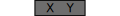
\includegraphics{graphics/basics/temporal_relations/equals}} \\
    $X$ starts $Y$ &    \texttt{X s Y} & \raisebox{-0.25\height}
    {
\includegraphics{graphics/basics/temporal_relations/starts}} \\
    $X$ during $Y$ &    \texttt{X d Y} & \raisebox{-0.25\height}
    {
\includegraphics{graphics/basics/temporal_relations/during}} \\
    $X$ ends $Y$ &      \texttt{X e Y} & \raisebox{-0.25\height}
    {
\includegraphics{graphics/basics/temporal_relations/ends}} \\
    % \bottomrule
\end{tabular}
\caption{Temporal relations of time spans, based on \cite{allen84}}
\label{tab:temporal_relations}
\end{center}
\end{table}

% paragraph temporal_relations (end)

% subsection model_of_historical_time (end)

% ------------------------------------------------------------------------------
\subsection{Presentation of Historical Time} % (fold)
\label{sub:presentation_of_historical_time}

In contrast to space, time does not have an intrinsic representation. However, the most common form to visualize cyclic time is on a cyclic display, e.g. a time wheel or a clock. Linear time is very often visualized on a \emph{timeline}. The purpose of a timeline is to show events as time points or processes as time intervals in chonological order. A timeline additionally shows time markers showing a certain date to support orientation. A timeline uses a certain time scale:

\begin{itemize}
  \item On a \emph{linear} timeline, the distance between any two time points is directly proportional to their actual temporal distance.
  \item A \emph{logarithmic} timeline uses a logarithmic function to scale the depicted time. Relative to a reference point on the timeline, e.g. the timeline center, the further away a time point, the further away its position on the timeline -- however, the distance between the time point and the reference point does not increasy linearily, but logarithmically. That means, events that are further away do not appear as far. This time scale accounts for logarithmic human perception: events that happened 20 years ago do not seem to be twice as long ago as events happening 10 years ago
  \cite{logorlinear}.
  \item A timeline can also have an \emph{irregular} scale, e.g. to have the same absolute distance of events on the timeline. This is useful if the distribution of the events on the timeline are far from homogeneous.
\end{itemize}

\begin{figure}[ht]
  \centering
  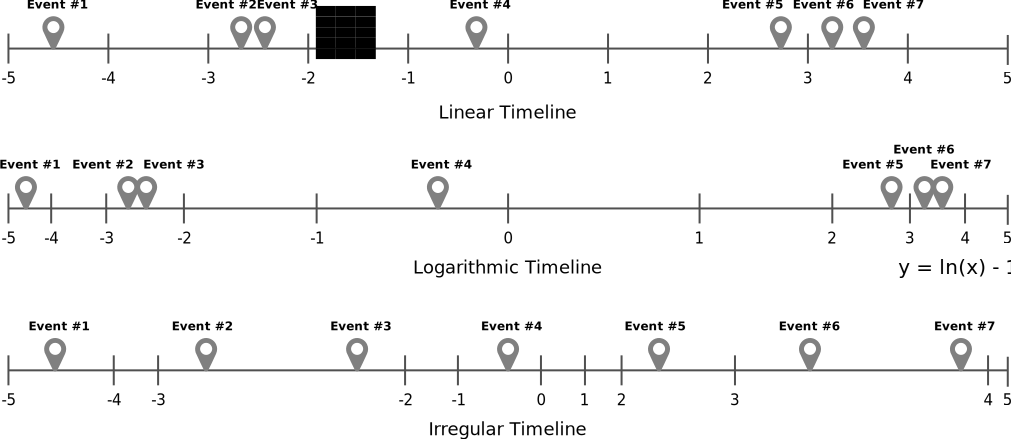
\includegraphics[width=0.8\textwidth]{graphics/basics/timelines/timelines}
  \caption{Comparison between a linear, a logarithmic and an irregular timeline}
  \label{fig:timelines}
\end{figure}

The visualization of time can be separate from the spatial dimension, according to the Triadic Framework, e.g. with a timeline. In another approach, space and time can also be coupled and displayed in the same presentation display, e.g. in a space-time cube \cite{haegerstrand1970}.


% temporal domain
%   linear time
%     time line
%     time series: graph (t,y coordinate system)
%     2.5D map: temporal dimension on z axis or on surface
%     space-time path
%   cyclic time
%     time series: polar diagram
%     time wheel
%   both
%     mono-temporal: one layer -> one time point
%     multi-temporal: one layer -> multiple time points
% \cite[p. 144]{ott2001time}

% subsection presentation_of_historical_time (end)

% section time_and_space (end)


% ==============================================================================
\section{Spatio-Temporal Data Models} % (fold)
\label{sec:spatio_temporal_data_models}
\begin{quoteit}
  ``Geography differs from geometry because \\
  in geography, space in indivisibly coupled with time''
\end{quoteit}
\hfill -- Don Parkes \& Nigel Thrift (1980)

A model tries to replicate a part of the real world. A data model abstracts a part of the world, identifies the most essential elements and their relation to each other. Historical Geographic Information Systems can be used to explain spatial-temporal phenomena in the real world. Therefore, it needs to handle the development of geo-objects and their attributes over time. Developments are driven by \emph{changes} to the state of an object.

Based on the theory of the \emph{Triadic Framework}, there are three components involved: space (3 dimensions), time (1 dimension) and attribute (multiple dimensions). All of these dimensions can change independently from each other
\cite[p. 53]{ott2001time}.
However, in order to trace spatial and attribute changes over time, the dimensions have to be related to each other.

% TODO: absolute time vs. relative time
% TODO: absolute space vs. relative space

Throughout the lifetime of a geo-object, it appears at some point, might undergo several changes and might disappear at some other time point. The data model has to be able to effectively and efficiently manage those changes. There are mainly two kinds: \emph{Discrete changes} are based on the idea of a \emph{state machine}: At any point in the lifetime, an object is in a certain state. It stays there until an event occurs that suddenly changes the object into a new state at a discrete time point. As an example, if an armistice agreement between two former war parties $A$ and $B$ contains a deal to cede parts of the territory of A to become territory of B, this territorial change is sudden. On a contrary, an object can gradually change according to a \emph{continuous process}, e.g. the change of the coastlines of landmasses
\cite{peuquet99}.

The spatio-temporal data models developed in the previous 30 years differ mostly in the organizing dimension: In \emph{location-based} models time is an attribute of a geo-object. On a contrary, \emph{time-based} approaches handle events and processes that change objects suddenly or gradually. \emph{Entity-based} models represent geo-objects as own entities. Spatial changes over time are related to these entities, but they are not attributes and therefore independent.


% The basis for all models is the concept of \emph{Time Geography} by
% \cite{haegerstrand1970}:
% Hägerstrand argued for an orthogonal relationship between time and space and that each object can be at one location only at one time. He furthermore visualized an objects development in a \emph{space-time path}. This section will introduce the most important \emph{spatio-temporal data models} (STDM) based on this idea that are releveant for the remaining parts of the thesis.
% TODO: version management (Wachowitz p 43)

This section introduces different spatio-temporal data models to maintain relations between time and space of an entity.

% ------------------------------------------------------------------------------
\subsection{Snapshot Model} % (fold)
\label{sub:snapshot_model}

One of the simplest, oldest and most frequently used models is based on the idea of \emph{snapshots}: At a certain time point $t_i$, a new layer gets created. It stores the full picture of the current state of all geo-objects
\cite{Langran1988frameworktgis}.

\begin{figure}[H]
  \centering
  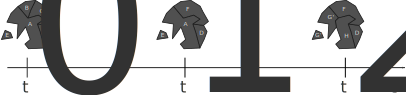
\includegraphics[width=0.8\textwidth]{graphics/basics/stdm/snapshot_model}
  \caption{The Snapshot Model by \cite{Langran1988frameworktgis}}
  \label{fig:snapshot_model}
\end{figure}

The model allows to retrieve the state of the system at a defined time point $t_i$. However, for all other time points $t \neq t_i$ that are not covered by a snapshot, it is impossible to retrieve the state of the system, because the data model does not record any changes. This is an integral problem of the model and can not be solved. The original model is also redundant, because objects that have not changed from one snapshot to the next one are duplicated. However, there have been improvements made, e.g. by \cite{armenakis92}.
Historical maps are examples for snapshots: They show the state of the world at one point in history, e.g. Europe 1919 and Europe 1945. However, with no additional information, it is impossible to deduct how Europe looked like in 1939. Therefore, this model is not suitable for the domain of this thesis.

% subsection snapshot_model (end)

% ------------------------------------------------------------------------------
\subsection{Simple Time-Stamping} % (fold)
\label{sub:simple_time_stamping}

This problem is solved by assigning a geo-object a period of existance by two additional attributes: at the \emph{start date} $t_{start}$ the object gets created and at the \emph{end date} $t_{end}$ it is ceased. If an object still exists its cessation date gets a special value, e.g. \texttt{NOW}
\cite{hunter90timestamping}.

\begin{figure}[ht]
  \centering
  
\includegraphics[width=0.8\textwidth]{graphics/basics/stdm/simple_time_stamping}
  \caption{The Simple Time-Stamping method by \cite{hunter90timestamping}}
  \label{fig:simple_time_stamping}
\end{figure}

The \emph{Simple Time-Stamping} method is also location-based and tracks discrete changes of objects. Given full and integer information, the state of the system at each time point $t_i$ can be retrieved: All geo-objects for which ~$t_{start} \leq t_i < t_{end}$~ are active, all others are inactive. However, this retrieval is cumbersome, because without efficient data structures every time the date changes, it has to be checked for each geo-object if its state has changed.

Another problem of the model is that it does not allow for tracing the development of objects in different states. As an example, at time point $t_1$ the geo-objects $B$ and $C$ cease and $G$ starts. Visually, $G$ is a successor of $B$ and $C$, but this historical relationship can not be deducted directly from the model. This shortcoming can be resolved by adding a reference to the predecessor and the successor of the object.

This model alone is not suitable for the domain of this thesis, because it is impossible to say what exactly has happened at a certain time point. Given the example above, it is unclear if two objects unified to a new one ($B+C \to G$) or if two are successors ($B \to G$) and one just stops to exist ($C \to \emptyset$). The model is also redundant: if a geo-object replaces another one ($B \to G$), then the end date of $B$ is the same as the start date of $G$.
% \cite[p. 46-47]{solana2014spatio}.

% subsection simple_time_stamping (end)

% ------------------------------------------------------------------------------
\subsection{Event-Based Spatio-Temporal Data Model} % (fold)
\label{sub:event_based_spatio_temporal_data_model}

A time-based approach addresses exactly those shortcomings: They explicitly represent events or processes in the data model and associate all objects that change according to them. One example of this approach is the \emph{Event-Based Spatio-Temporal Data Model} (ESTDM) for geospatial raster data by
\cite{peuquet95}.

At one defined time point $t_b$, a snapshot gets stored. This \emph{base map} contains the current state of the map, i.e. the current value of each raster cell \texttt{(x,y)}. From that moment on, the system stores events that change the values of certain cells. Such an event has a time stamp (\texttt{t}) and a list of components associated with it. A component represents a new value (\texttt{v}) and knows which raster cells (\texttt{x}, \texttt{y}) change their value to \texttt{v}.

The method uses the following data structures: a header file contains information about the thematic domain, a pointer to the base map and to the first and last element of the event list. This doubly-linked list stores all events chronologically. Therefore, each event knows its preceding and succeeding event via a \texttt{prev} respectively \texttt{next} pointer.
% TODO: graphic

If the time point of an event is reached, all its components are executed, i.e. the relevant raster cells change their value. The system follows the \texttt{next} pointer to know which event is waiting to be executed next. Since a change is relative to the previous change, not to the base map, change tracking is efficient.

The concept of the ESTDM suits the problem domain really well: An historical event changes the geometry of certain objects suddenly. The model explicitly represents these discrete changes. However, it does not work for vector data. The authors have explicitly stated that ``the design of such a [vector-based] model is not seen as a straightforward task'', because of the problem ``how to maintain the integrity of spatial topology as it changes [...] The solution will require a more complex definition of components within individual events''
\cite[p. 21]{peuquet95}.

% Also, just like the Simple Time-Stamping method, this model is only suitable for discrete but not for gradual changes. This problem is solved in the \emph{ObjectOriented geomorph} model by \cite{raperlivingstone95}.

% subsection event_based_spatio_temporal_data_model (end)

% ------------------------------------------------------------------------------
\subsection{Three-Domain Model} % (fold)
\label{sub:three_domain_model}

An event-based STDM for vector geometry including lines and polygons has to answer the following questions: What uniquely identifies a geo-object? What kind of spatial, topological and attribute changes can happen to an object? Which of these maintain the identity and which create a new object? This problem is addressed in the \emph{Three-Domain Model} by \cite{yuan96threedomain, yuan96temporal}. The model is based on abstract entities that represent a spatio-temporal object. It handles the three domains identity, space and time separately:
\begin{itemize}
  \item The \emph{semantic domain} holds an entity uniquely identifiable. An object in this domain corresponds to a human concept, e.g. a ``country''.
  % It handles attributes of the area, but not the spatial and temporal properties.
  \item The \emph{spatial domain} represents geospatial objects in vector format, e.g. a polygon describing the territory of a country.
  \item The \emph{temporal domain} stores all temporal objects, e.g. time points of an historical events, or time intervals of a war.
\end{itemize}

The model is not specific, but more a general abstract framework to handle space, time and identity. This makes the model very flexible, e.g. it can handle discrete and continuous changes, relative and absolute time, world and database time. One limitation of the model is that it only traces spatial attributes over time. In an alternative model by \cite{claramunt95timeingis}, the \emph{thematic domain} is added to fully describe a spatio-temporal object and trace also aspatial attributes that can change over time, e.g. the name of an entity.



Since countries, their territories and attributes can change independently over time, the data model used in this thesis will be built on top of the Three Domain Model.

% subsection three_domain_model (end)

% ------------------------------------------------------------------------------
\subsection{History Graph Model} % (fold)
\label{sub:history_graph_model}

Most of the data models introduced so far cover only static changes of geo-objects. \cite{renolen96} identified three different types of temporal behaviour of changing objects:
\begin{compactitem}
  \item Dynamic objects that change continuously.
  \item Static objects that change according to events with duration (processes).
  \item Static objects that change according to sudden events.
\end{compactitem}

Based on this observation he developed a data model that can handle all three kinds of temporal behaviour: The \emph{History Graph Model}. It manages objects and events separetly from each other. An object can only be in three different states:
\begin{enumerate}
  \item An object is \emph{static}, if it currently does not change. This is called an \emph{object version}. The version has an interval associated to it representing the duration of the object version, until it changes the next time. If the object is dynamic and changes continuously, the duration is zero.
  \item If an object is currently \emph{changing}, it is in an \emph{object transition}. The transition has an associated interval as well, whose duration is zero if it is a sudden change. Additionally, a transition links the relevant objects to each other creating a historical predecessor-successor-relationship.
  \item An object that is currently not active, is \emph{ceased} and not visible on the map.
\end{enumerate}

The history of a geo-object is a chronologically ordered set of versions and transitions, that can be visualized in a graph (see figure \ref{fig:history_graph_model}).

\begin{figure}[H]
  \centering
  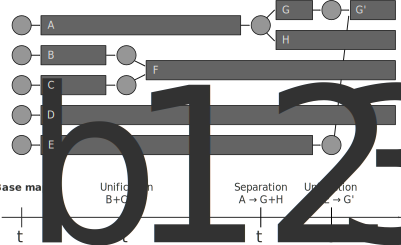
\includegraphics[width=0.8\textwidth]{graphics/basics/stdm/history_graph_model}
  \caption{The History Graph model}
  \label{fig:history_graph_model}
\end{figure}

The model defines six basic types of temporal changes that can happen (see figure \ref{fig:history_graph_changes}):
\begin{compactitem}
  \item \textbf{Creation}:           A new object is created.
  \item \textbf{Alteration}:         A property of an object (e.g. geometry) changes.
  \item \textbf{Cessation}:          An object is ceased.
  \item \textbf{Reincarnation}:      An object that has previously been ceased is recreated.
  \item \textbf{Split/Deduction}:    An object is divided into two or more new objects or one or more objects are deducted from an existing one.
  \item \textbf{Merge/Annexation}:   Two or more objects are joined together to a new object or one or more objects are annexed to another object.
\end{compactitem}

\begin{figure}[ht]
  \centering
  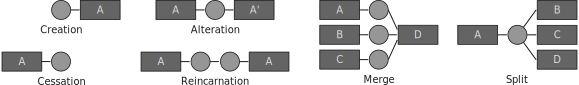
\includegraphics[width=0.8\textwidth]{graphics/basics/stdm/history_graph_changes}
  \caption{Types of changes in the History Graph model}
  \label{fig:history_graph_changes}
\end{figure}

The History Graph model can be seen as an extension to the ESTDM. It combines the advantages of event-based and entity-based spatio-temporal data models, supports discrete and continuous changes and relative and absolute time. The main improvement is that the historical development of a geo-object can directly be derived from the model, because objects are linked to their precedessors and successors --- the History Graph Model can tell a story. This is the reason why this model is particularly suitable for the work of this thesis.

% subsection history_graph_model (end)

\vspace{1em}
Other popular spatio-temporal data models that are not covered in this work, because they were not seen as relevant for the domain, include the \emph{Space-Time Composite} model, the \emph{Grid Model} and the \emph{Amendment Vector Model}. Overviews about these and other spatio-temporal data models can be found in \cite{zhao11}, \cite{pelekis04stdms} and \cite{peuquet99}.

% section spatio_tempora_data_models (end)


% ==============================================================================
\section{Database Management Systems} % (fold)
\label{sec:database_management_systems}

Information systems use databases for managing the data. A \emph{Database Management System} (DBMS) is a software system for the administration of data, mainly storage and retrieval. There are mainly two types of DBMS: the oldest and most common ones are \emph{Relational DBMS}. \emph{Object-Oriented DBMS} werde developed to adapt concepts of object-oriented programming into the database world. The combination of both approaches are \emph{Object-Relational DBMS}.

% ------------------------------------------------------------------------------
\subsection{Relational Database Management Systems} % (fold)
\label{sub:relational_database_management_systems}

RDBMS are built upon the concept of \emph{entitities}, e.g. an \texttt{HistoricalCountry}, with \emph{attributes}, e.g. \texttt{name} and attribute values of a simple data type, e.g. the character string \texttt{"Germany"}. Entities are represented in a table with one row for each \emph{tuple} and one column for each attribute. An entity has one attribute that unambiguously identifies each tuple, the \emph{primary key}, mostly a contiguous number.

Entities can be related to each other in three different kinds of \emph{relations}:
\begin{compactenum}
  \item[\texttt{1:1}] Direct attributional relation, e.g. one country has one head of state and vice versa.
  \item[\texttt{1:n}] One-to-many relation, e.g. one country can have many cities, but each city can belong to only one country.
  \item[\texttt{m:n}] Many-to-many relation, e.g. one country can have many rivers, but each river can also flow through multiple countries.
\end{compactenum}

Entities and their relations are visualized in an \emph{Entity-Relationship Model} (ER model). Data can be retrieved from and entered into a relational database using the \emph{Structural Query Language} (SQL). The query to get the names of cities in \texttt{Germany} in alphabetical order is:

\vspace{-1em}
\begin{verbatimtab}
  SELECT     city.id, city.name
  FROM       (city JOIN country ON city.country = country.id)
  WHERE      country.name = "Thüringen"
  ORDER BY   city.name
\end{verbatimtab}
\vspace{-1em}

The first RDBM developed was \emph{Oracle}, released in 1979 \cite{oracleDB}. Since then, the concept has been established as the state-of-the-art for databases. An example for a popular RDBMS used for Web-bases systems is \emph{MySQL}, the ``world's most popular open source database''
\footnote{
  \emph{MySQL :: About MySQL},
  URL: \url{https://www.mysql.com/about/},
  last access: 31.10.2015
}.


% subsection relational_database_management_systems (end)

% ------------------------------------------------------------------------------
\subsection{Object-Oriented Database Management Systems} % (fold)
\label{sub:object_oriented_database_management_systems}

One problem with RDBMS is that attributes can only be assigned simple data types. Developers using object-oriented programming need to map the objects used in the application to tuples in the relational database -- and vice versa data from the database needs to be transformed to objects in the application. This process can be cumbersome. OODBMS have been developed to address this problem and adopt the concepts of object-oriented programming for database management purposes \cite{oodbms}.

\begin{itemize}
  \item \emph{Classes} are the structured representation of things in the real world of the same kind, with the same properties, e.g. a country, having a name and a territory. Classes in OODBMS relate to Entities in RDBMS.
  \item An \emph{object} is an instance of a class, one specific thing with defined properties, e.g. the country of Germany with its territory. This correlates to a tuple in RDBMS.
  \begin{itemize}
    \item The \emph{attributes} of an object can not just be of a simple data type, but also instances of other classes, e.g. \texttt{country.territory} can be a \texttt{polypolygon} object. These complex data types are a major improvement compared to RDBMS.
    \item Objects also have \emph{methods} that can be called to do something with the object, e.g. \texttt{territory.getArea()} calculates the area size of a country.
  \end{itemize}
  \item The internal state of an object can not be accessed from the outside. Methods are the only way to interact with an object. This is called \emph{encapsulation} and maintains control over what can be done to and with an object and prevents corruption.
  \item According to the concept of \emph{inheritance}, classes can be hierarchically structured, whereas the attributes and the methods of a \emph{base class} are inherited to its \emph{derived class}. As an example, an \texttt{Area} has a \texttt{name}, a \texttt{territory} and the method \texttt{getArea()} associated to it. A \texttt{Country} can be derived from the \texttt{Area}, inheriting both attributes and the method. Additionally, it can get an attribute \texttt{head\_of\_state}, which is specific to \texttt{Country}, but not to \texttt{Area}. The class \texttt{Ocean} can just as well be derived from \texttt{Area}.
  \item An associated concept is \emph{polymorphism}: The same function can be called on different objects and the return value will be of the same type. However, internally it might be calculated differently. As an example, consider the classes \texttt{Polygon} and \texttt{Polypolygon}, both inherited the method \texttt{getArea()} from their base class \texttt{Geometry}. Whereas a polygon calculates its area directly based on its geometry, a polypolygon internally calles the function \texttt{getArea()} on all its associated polygons and sums up their areas.
\end{itemize}

OODBMS support all those concept and allow to store the objects used in the application directly in the database. Additionally, objects from the database can be accessed directly, there is no need for an additional query language \cite{oodbms}.

% subsection object_oriented_database_management_systems (end)

% ------------------------------------------------------------------------------
\subsection{Object-Relational Database Management Systems} % (fold)
\label{sub:object_relational_database_management_systems}

ORDBMS combine the advantages of both worlds. Internally, it uses the established and efficient relational database for the data storage. The database model and the interaction with the data happens in an object-oriented way while supporting all of the concepts mentioned in the previous subsection \ref{sub:object_oriented_database_management_systems}. The most popular ORDBMS example for Web-based systems is \emph{PostgreSQL}, ``the world's most advanced open source database''
\footnote{
  \emph{PostgreSQL: About},
  URL: \url{http://www.postgresql.org/about/},
  last access: 31.10.2015
}.

% subsection object_relational_database_management_systems (end)

% ------------------------------------------------------------------------------
\subsection{Spatio-Temporal Databases} % (fold)
\label{par:spatial_databases}

Databases for HGIS have to deal with spatial, temporal and attribute data. According to the Triadic Frame, these aspects should be modeled separately from each other, as they can change independently.

% - - - - - - - - - - - - - - - - - - - - - - - - - - - - - - - - - - - - - - -
\paragraph{Spatial data} % (fold)
\label{par:spatial_data}

can easily become very large, because of the mass of very precise coordinate data. \emph{Spatial databases} are specialized to work with spatial data: they process the data effieciently and to provide general data types, such as \texttt{Point} or \texttt{Polygon} and methods, e.g. to calculate the area or the distance between two points. \emph{PostGIS}
\footnote{
  \emph{PostGIS},
  URL: \url{http://postgis.net/},
  last access: 31.10.2015
}
is an extension for PostgreSQL that is especially utilized for handling spatial data.

% paragraph spatial_data (end)


% - - - - - - - - - - - - - - - - - - - - - - - - - - - - - - - - - - - - - - -
\paragraph{Temporal data} % (fold)
\label{par:temporal_data}

usually relates to events and processes. It is defined either by a time point or a time interval which is again defined by two time points. This is called a \emph{bitemporal} element. A time point can be modeled in the database as an attribute of the complex \texttt{Date} type. For relational databases that only support simple data types, the date can be stored as a string or be expressed with a \texttt{long} integer (64 bit) $\forall n \in \mathbb{N}: n \in [-2^{63}~..~2^{63}-1]$) determining the number of milliseconds since \nth{1} January 1970 (UNIX time) \cite{timeInRDBMS}. SQL was extended by features to handle time in a database, e.g. \emph{SQL/MM} \cite[chapter 6]{peuquet99}.

% paragraph temporal_data (end)

% - - - - - - - - - - - - - - - - - - - - - - - - - - - - - - - - - - - - - - -
\paragraph{Object-Oriented Spatio-Temporal Database Models} % (fold)
\label{par:object_oriented_spatio_temporal_database_models}

The question is: How to implement the spatio-temporal data modles introduced in section \ref{sec:spatio_temporal_data_models} in a relational, object-oriented or object-relational database management system introduced in this section? While the implementation depends on the data model, there are common concepts and isses that have to be addressed.

When storing time related data, it is important to distinguish between the time that was true in reality (\emph{valid time} or \emph{world time}) and the time it was stored in the database (\emph{transaction time} or \emph{database time}). A property of spatio-temporal database models is whether valid and transaction time are supported.

Object-oriented concepts are more appropriate than the concept of relational databases, because of the complex nature of spatio-temporal data \cite[section 3.9]{pelekis04stdms}. One of the first concepts was the concept of a \emph{spatio-temporal object} combining geometrical and bitemporal properties in one object \cite{worboys90stdm}.

A similar approach by \cite{raza12} is the \emph{Spatio-Temporal Data Type} (STT). Time is not considered an attribute of space, but a separate class. They are aggregated in the \texttt{SpatioTemporal} class, using both spatial and bitemporal attributes. The model also provides spatio-temporal operators, e.g. \texttt{STT\_intersects} returns \texttt{true} if two \texttt{SpatioTemporal} objects intersect in time and space, i.e. their geometries intersect and the time intervals in which they are active overlap. These operators are very helpful when analyzing spatio-temporal data or checking for data integrity.

% paragraph object_oriented_spatio_temporal_database_models (end)

% - - - - - - - - - - - - - - - - - - - - - - - - - - - - - - - - - - - - - - -
\paragraph{Version management} % (fold)
\label{par:version_management}

An issue is how to perform retrospective updates. Given a database model that stores objects that are created, updated and destroyed by events. Object $X$ is created at time point $t_x$. At time point $t_y$, $X$ gets destroyed and replaced by object $Y$. If a new change that updates $X$ to $X'$ gets inserted at time point $t_u$ in between, i.e. $t_x < t_u < t_y$, then the event at time point $t_y$ is not correct anymore, because object $X$ does not exist. The question is how to maintain data integrity on insertion, update and deletion from a spatio-temporal database? This issue has to be addressed using formal logic for temporal reasoning
\cite[section 6]{peuquet99}.

% One approach to handle this issue is \emph{version management}, introduced by
% \cite WH94
% There are \emph{object version} and \emph{object configuration}. The concept is based on four premises:
% \begin{compactenum}
%   \item Each object must have an initial version.
%   \item The versions of an object are hierachically structured.
%   \item One object version relates to exactly one object instance and vice versa.
%   \item There is always one current version of an object.
% \end{compactenum}

% Throughout time, a set of interrelating object versions is created. They are handled by four update procedures that create new object versions:
% \begin{compactenum}
%   \item Create of a new object.
%   \item Clone an existing object.
%   \item Update spatial attributes of an existing object (geometric change).
%   \item Update aspatial attributes of an existing object (thematic change).
% \end{compactenum}

% paragraph version_management (end)


% \cite[p. 69]{ott2001time}.

% section database_management_systems (end)

\vspace{2em}

transition to concept chapter
%!TEX root = ../masters_thesis.tex

\chapter{Development} % (fold)
\label{cha:development}

The aim of this thesis is to create a Historical Geographic Information System to visualize and edit the evolution of countries in time and space. This is a complicated task, because both the reality and the human using the system are complex. For such complex applications the methodologies of \emph{Human Centered Design} are promising to create an interface that humans can easily understand.

The development process is iterative and divided in several phases. In each phase creates a prototype or the interface that gets closer to the final solution by increasing the fidelity of the prototype. A phase starts with an initial set of requirements. In multiple iterations, a prototype is developed that solves the problem. Each iteration has four steps: The requirements for the system are analyzed in the \emph{planning} step. Afterwards, they translated into an abstract \emph{design} which is realized in a specific \emph{implementation} of the prototype. Finally, this prototype is tested with humans to find out how well it works. Based on the results of this \emph{testing} step, the requirements are updated and the next iteration starts. This is repeated until a version of the interface is created that sufficiently solves the problem. Then the fidelity is increased, starting the next development phase. The five phases in this thesis are shown in figure \ref{fig:hcd}.

\begin{figure}[H]
  \vspace{1em}
  \centering
  \includegraphics[width=0.9\textwidth]{graphics/development/hcd}
  \caption{Human Centered Design process with five project phases}
  \label{fig:hcd}
\end{figure}

\newpage
\begin{compactenum}
  \item \textbf{Idea}: The initial idea how to edit and visualize the history of countries.
  \item \textbf{Paper Prototype}: The concept of the interface realized and tested on paper.
  \item \textbf{Mockup Prototype}: The concrete workflow developed in a slide-based presentation.
  \item \textbf{Web-Based Prototype}: The final version developed in a Web application.
  \item \textbf{Extensions}: Design approaches to account for the uncertain nature of history.
\end{compactenum}

There are several models involved in the development of the software, each of them has to be developed or analyzed separately. The \emph{data model} is an abstraction and simplification of the real world. The \emph{Hivent Model} developed in this thesis is explained in the first section \ref{sec:hivent_model} of this chapter. It follows the method to \emph{edit} the spatio-temporal data in the system in section \ref{sec:editing_hivent_data}. In iteractive computer systems, the \emph{mental model} is the representation in the mind of the human about how the interface should work -- the \emph{conceptual model} describes the way the interface actually works. The goal of Human Centered Design is to match the conceptual model to the mental model. Section \ref{sec:user_interface_design_process} outlines the gradual design process to reach this goal. In the application, the data model is implemented in the \emph{database model}. The task for the \emph{computational model} is to translate between the database model and the conceptual model. The HistoGlobe application, including the database and computational model, is introduced in the last section \ref{sec:application} of this chapter.

\begin{figure}[H]
  \vspace{1em}
  \centering
  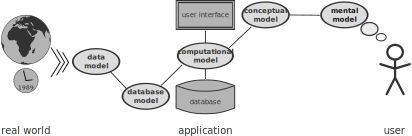
\includegraphics[width=0.8\textwidth]{graphics/development/models}
  \caption{Relevant models for an information system}
  \label{fig:models}
\end{figure}

% ==============================================================================
%!TEX root = ../masters_thesis.tex

\section{Hivent Model} % (fold)
\label{sec:hivent_model}

This section proposes the spatio-temporal \emph{Hivent model} to represent the history of countries in time and space. \emph{Hivent} is an acronym for \emph{\textbf{Hi}}storical e\emph{\textbf{vent}} and is the main element of the data model. In section \ref{sec:spatio_temporal_data_models}, different spatio-temporal data models were introduced: The \emph{Snapshot} model is unsuitable for the problem space. \emph{Simple time-stamping} is helpful to link countries to their history, but it does not explicitly model historical changes, which is required. For that purpose, the \emph{ESTDM} was developed, but since it only works for raster data, it does not match the problem space. The \emph{History Graph} model fills this gap and additionally introduces temporal changes and their influences on geographic entities directly in the model. Finally, the \emph{Three-Domain} model presents a helpful concept to separate the spatial, temporal and thematic dimension of a spatio-temporal object.

The Hivent model is constructed from components of some of these models. It is event-based and supports vector data. It is organized in four domains and allows to visualize data on a graph.
Section \ref{sub:elements} introduces the main elements of the Hivent model. Afterwards, the basic axioms and assumptions are defined in section \ref{sub:preconditions}. A major contribution of this thesis is proposed in section \ref{sub:hivent_operations}: the set of five \emph{Hivent operations} that describe all possible changes of countries in time and space.
Section \ref{sub:histograph} presents the \emph{HistoGraph}, a non-spatial visualization of historical developments.

% ------------------------------------------------------------------------------
\subsection{Elements} % (fold)
\label{sub:elements}

% - - - - - - - - - - - - - - - - - - - - - - - - - - - - - - - - - - - - - - -
\paragraph{Hivents} % (fold)
\label{par:hivent}

represent historically significant happenings, e.g.\ a treaty, bill or declaration.
An Hivent happens at one particular point in time and space and is therefore the main organizing element of the eponymic data model.
The focus in this work is on events that influence the geopolitical situation on Earth.

% paragraph hivent (end)

% - - - - - - - - - - - - - - - - - - - - - - - - - - - - - - - - - - - - - - -
\vspace{-1em}
\paragraph{Areas} % (fold)
\label{par:area}

represent one identical current or historical country. They are abstract entities on the map with a \emph{name} and a \emph{territory}. In the real world, a country has a common \emph{short name}, e.g.\ ``Germany'' and a potentially longer \emph{formal name}, e.g.\ ``Federal Republic of Germany''. Both attributes are part of the Area model. The \emph{territory} of the Area is described by a polypolygon, a set of weakly simple polygons to account for enclaves and exclaves (see section \ref{ssub:vector_model}). The polylines of a polygon consist of an ordered set of points that represent the borders of the country.

% paragraph area (end)

% - - - - - - - - - - - - - - - - - - - - - - - - - - - - - - - - - - - - - - -
\vspace{-1em}
\paragraph{Historical Changes} % (fold)
\label{par:historical_changes}

The idea of the Hivent model is that Areas can change over time. This happens via \emph{historical changes} that are part of exactly one Hivent. Throughout the lifetime of an Area, it is created at some point $t_s$, its territory and short name can change multiple times $t_i: t_s < t_i$ and at some point $t_e: t_s < \forall t_i < t_e$ it may be deleted.
Each Area is \emph{uniquely identified by its formal name}. That means as soon as the formal name of an Area changes, it is considered a ``new'' Area.
Since all changes in this model are sudden, there are only two possible states an Area can be in: It is \emph{active}, if at the current point in time it is historically existing, otherwise it is \emph{inactive}.

\begin{figure}[H]
  \vspace{1em}
  \centering
  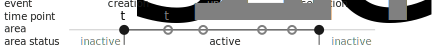
\includegraphics[width=0.9\textwidth]{graphics/development/hivent_model/area_states}
  \caption{Three event types that change Areas, resulting in two different area states}
  \label{fig:area_states}
\end{figure}

Historical changes and Areas are mutually linked, i.e.\ an Area keeps references to the changes creating, updating and deleting it and a historical change stores a set old Areas that are deleted, a set of new Areas that are created and a set of update Areas that are manipulated in the change.

% paragraph historical_changes (end)

% - - - - - - - - - - - - - - - - - - - - - - - - - - - - - - - - - - - - - - -
\paragraph{Four-Domain model} % (fold)
\label{par:four_domain_model}

Following the idea of the Three-Domain model and its extension introduced in section \ref{sub:three_domain_model}, the Hivent model is as well organized by four domains that are modeled independently from each other:

\begin{compactitem}
  \item The \emph{semantic domain} holds the Area uniquely identifiable is represented by its formal name.
  \item The \emph{spatial domain} is expressed by the territory of the Area that is visible on the map.
  \item The \emph{thematic domain} is represented by the short name of the Area.
  \item The \emph{temporal domain} is the entirety of all historical changes associated with the Area.
\end{compactitem}

The main difference between the spatial and the thematic domain is that there is no relation between the names of two Areas. While the intention is questionable, there could potentially be two Areas active at the same time with the same name. The update of the name of one Area is independent from any other Area. This is not true for the spatial domain: The territories of two Areas are highly related to each other. Geospatially, each territory has at least one neighbor and two neighbors share the same border. An update of the territory of one Area results in the update of at least one other territory.

% paragraph four_domain_model (end)

% subsection section area (end)

% ------------------------------------------------------------------------------
\subsection{Preconditions} % (fold)
\label{sub:preconditions}

\begin{quoteit}
  In the beginning God created the heavens and the Earth \\
  Now the Earth was formless and empty [...] \\
  And God said, “Let there be light” --- and there was light.
\end{quoteit}
\hfill -- Genesis 1:1, The First Book of Moses, Old Testament
\vspace{1em}


There are five axioms and two assumptions the Hivent model is based on. The theoretical foundation is the model of the Earth and its curved surface that can be projected onto a two-dimensional map using a map projection, as introduced in sections \ref{sub:geospatial_data}.

\newtheorem{invariant_surface}[assicounter]{Axiom}
\begin{invariant_surface}
\label{axm:invariant_surface}
  The Earth's surface has an invariant area size, i.e.\ it does not change over time.
\end{invariant_surface}

\vspace{-2.0em}
\newtheorem{area_on_surface}[assicounter]{Axiom}
\begin{area_on_surface}
\label{axm:area_on_surface}
  Each Area in the spatio-temporal system is located directly on the surface of the Earth.
\end{area_on_surface}

These axioms set the spatial foundation of the system: a constant dimension of the map and Areas covering the map. The basis of the temporal part of the system is content of the following axioms:

\vspace{-1.0em}
\newtheorem{initial_configuration}[assicounter]{Axiom}
\begin{initial_configuration}
\label{axm:initial_configuration}
  The spatio-temporal system is initialized at $t_0$. At this initial state, exactly one Area exists. It is denoted by $\Omega$ and is referred to as the \emph{universe} Area. It has no name and its territory covers the whole surface of the Earth.
\end{initial_configuration}

\vspace{-2.0em}
\newtheorem{historical_change}[assicounter]{Axiom}
\begin{historical_change}
\label{axm:historical_change}
  At each point $t_i \geq t_0$, multiple historical changes can be introduced.
\end{historical_change}

\vspace{-2.0em}
\newtheorem{unique_coverage}[assicounter]{Axiom}
\begin{unique_coverage}
\label{axm:unique_coverage}
  At each point $t_i \geq t_0$, each point on the surface of the Earth is covered by exactly one territory of exactly one Area.
\end{unique_coverage}

As defined in section \ref{par:area}, a historical change can create, manipulate and delete Areas on the Earth's surface. According to axiom \ref{axm:unique_coverage}, each change introduced in the system must maintain the spatial integrity on the map, i.e.\ if an Area is created on the map, the Area claiming this territory before has to secede it.

Formally, it can be said that each change consists of three sets of Areas: the old Areas $A$ that are deleted, the new Areas $B$ that are created and the Areas $C$, whose properties are updated in the change. Each $A_i \in A$ and $B_i \in B$ has a territory $A_i^T$ respectively $B_i^T$. Each $C_i \in C$ has an old territory $C_i^{OT}$ that is updated with the new territory $C_i^{NT}$. Each change introduced in the spatio-temporal system must maintain the spatial integrity of axiom \ref{axm:unique_coverage}. Therefore, the total size of the territories before the change and after the change must be the same:

\vspace{-.5em}

\[
  \left|\bigcup\limits_{i=1}^n A_i^T\right|
  +
  \left|\bigcup\limits_{i=1}^n C_i^{OT}\right|
  ~=~
  \left|\bigcup\limits_{i=1}^n C_i^{NT}\right|
  +
  \left|\bigcup\limits_{i=1}^n B_i^T\right|
\]

\vspace{.5em}

This behavior is based on to the law of conservation of energy in physics: energy in a closed system can only be transformed from one form to another, from one object to another -- but the total energy in the system is preserved at any time. In this spatio-temporal system, the total size of the territory of the Earth is preserved, but it is distributed among the active Areas in the system.

The first changes introduced in the system at $t_0$ are the creation of all bodies of water, including the oceans and lakes, denoted as $W$. Each Area $W_i \in W$ is created with their name and territory cut out of $\Omega$. The result is that after $t_0$, the map is divided into water ($W$) and land ($\Omega$). Land can at any point in time be either \emph{claimed}, i.e.\ it is currently occupied by the territory of exactly one active Area, or \emph{unclaimed}, i.e.\ belonging to $\Omega$.
% It is a subtractive data model, because each new Areas territory is cut out of $\Omega$.

\begin{figure}[ht]
  \centering
  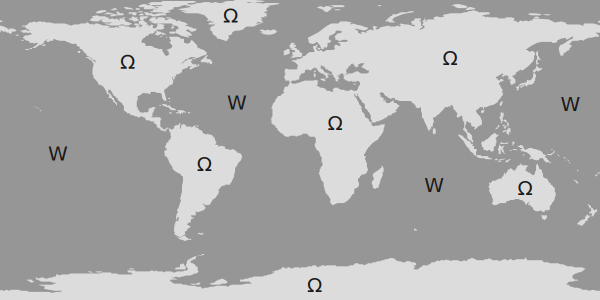
\includegraphics[width=0.6\textwidth]{graphics/development/hivent_model/init_map}
  \caption{The initial state of the world map at $t_0$}
  \label{fig:init_map}
\end{figure}

In the real world, the name of a country changes according to sudden events, e.g.\ a declaration or a governmental bill. The territory can change either because of geographical processes, e.g.\ the sea level rise influencing the coastlines, or according to a historical event, e.g.\ a treaty shifting a border between two countries. The Hivent model is based on two assumptions that simplify the model and keep the problem space clear:

\vspace{-0.0em}
\newtheorem{coastline_territory}[assicounter]{Assumption}
\begin{coastline_territory}
\label{axm:coastline_territory}
  The territory of a country stops at the coastline.
\end{coastline_territory}

\vspace{-1.5em}
\newtheorem{constant_coastlines}[assicounter]{Assumption}
\begin{constant_coastlines}
\label{axm:constant_coastlines}
  The coastlines have not changed over time.
\end{constant_coastlines}

Both assumptions are wrong. The territory of a country stretches into international water, as explained in section \ref{sub:territory_of_a_country}). Coastlines are constantly changing and so does the distribution of land and water on Earth. However, these assumptions allow the Hivent model to focus only on discrete historical changes. It is subject to future work to extend the model to account for long-term processes, e.g. the continental drifts of tectonic plates. For now, the temporal behavior of an Area in the Hivent model can be described as a \emph{static object that changes according to sudden events}.

% subsection preconditions (end)

% ------------------------------------------------------------------------------
\subsection{Hivent Operations} % (fold)
\label{sub:hivent_operations}

Respecting the preconditions, there are several different types of historical changes that transform a set of old Areas $A$ to a set of new Areas $B$ and update a set of Areas $C$. However, each possible historical change can be expressed with only one of five \emph{Hivent operations}. Four of them change the identity of at least one Area and therefore establish historical predecessor-successor-relationships. These relationships are always symmetric, i.e.\ if one old Area is replaced by one new Area, the old Area is the historical predecessor of the new Area and vice versa. The last operation changes a non-spatial property of an Area and is therefore identity-preserving.

\newpage
\begin{description}

  \item[UNI -- Unification]
  A set of old Areas unifies to one new Area. The old Areas are deleted, becoming the historical predecessors of the new Area. The territory of this new Area is the union of the territories of the old Areas. The new Area receives a new name. \\[0.25em]
  \begin{footnotesize}
    In 1922, the Russian SFSR, the Transcaucasian SFSR, the Ukrainian SSR and the Byelorussian SSR unified and formed the Union of Soviet Socialist Republics (USSR).
  \end{footnotesize}

  \item[INC -- Incorporation]
  One or more old Areas are incorporated into another Area that stays active. Its territory is enlarged by the union of the territories of the old Areas. The old Areas are historical predecessors of the Area that stays active. \\[0.25em]
  \begin{footnotesize}
    In 1990, the territory of the German Democratic Republic (East Germany) became part of the Federal Republic of Germany (West Germany). Although this event is known as the \emph{German Reunification}, it is historically an incorporation of East Germany into West Germany \cite{incorporationEastWestGermany}.
  \end{footnotesize}

  \item[SEP -- Separation]
  As the inverse of unification, one old Area is separated into multiple new Areas. Each new Area gets a part of the territory of the old Area, receives a new name, and has the old Area as its only historical predecessor. \\[0.25em]
  \begin{footnotesize}
    In 1993, the Czech and Slovak Federal Republic, commonly known as Czechoslovakia, dissolved into present-day Czech Republic and Slovak Republic, creating two new countries out of one old.
  \end{footnotesize}

  \item[SEC -- Secession]
  As the inverse of incorporation, one or more new Areas are ceded from a previously existing Area that stays active. Each new Area gets a new name, receives the previously existing Area as the only historical predecessor and a part of its territory. \\[0.25em]
  \begin{footnotesize}
    In 2008, the Republic of Kosovo declared independence from Serbia and has since then partially received international recognition. Serbia stays a country, keeping its name, but ceding a part of its territory to Kosovo.
  \end{footnotesize}

  \item[NCH -- Name Change]
  An Area changes its short name but preserves its formal name and identity. \\[0.25em]
  \begin{footnotesize}
    A recent change happened on 05.05.2016: The cabinet of Czech Republic approved that the country will now officially be called ``Czechia''. However, the formal name stays ``Czech Republic'', which preserves its identity.
  \end{footnotesize}
\end{description}

\vspace{1.5em}
\begin{table}[H]
\begin{center}
\begin{tabular}{cx{2.5cm} cx{2.5cm} cx{2.5cm} cx{2.5cm} cx{2.5cm}}

  \texttt{UNI} & \texttt{INC} & \texttt{SEP} & \texttt{SEC} & \texttt{NCH} \\
  Unification & Incorporation & Separation & Secession & Name Change \\[1em]

  
\includegraphics{graphics/development/hivent_model/operations/UNI} &
  \includegraphics{graphics/development/hivent_model/operations/INC} &
  
\includegraphics{graphics/development/hivent_model/operations/SEP} &
  \includegraphics{graphics/development/hivent_model/operations/SEC} &
  
\includegraphics{graphics/development/hivent_model/operations/NCH} \\

\end{tabular}
\caption{The five Hivent operations}
\label{tab:hivent_operations}
\end{center}
\end{table}

% subsection hivent_operations (end)

% ------------------------------------------------------------------------------
\subsection{HistoGraph} % (fold)
\label{sub:histograph}

Based on the idea of the History Graph model, introduced in section \ref{fig:history_graph_model}, the linguistically and conceptually related \emph{HistoGraph} visualizes the temporal development of countries. The edges of the graph represent an Area, the nodes a Hivent operation. The graph shows the predecessor-successor-relationships between Areas. As previously explained in section \ref{par:historical_changes}, an Area keeps references to the historical changes creating, updating and ceasing it. These changes themselves are linked to their old and new Areas. Therefore, each Area indirectly knows their successors and predecessors. The two-dimensional HistoGraph has a horizontal orientation. The x-axis refers to one point in time, the y-axis has no spatio-temporal relation. The graph uses the visualization approach of the five Hivent operations in table \ref{tab:hivent_operations}, including the following symbols:

\begin{table}[H]
\begin{center}
\begin{tabular}{c l l}

  \raisebox{3.5\height}

  \raisebox{-0.2\height}
  {
\includegraphics[width=10px]{graphics/development/hivent_model/histograph/circle_filled}}
  & Identity-changing Hivent operation
  & \texttt{UNI}, \texttt{INC}, \texttt{SEP}, \texttt{SEC} \\

  \raisebox{-0.2\height}
  {
\includegraphics[width=10px]{graphics/development/hivent_model/histograph/circle_unfilled}}
  & Identity-preserving Hivent operation
  & \texttt{NCH} \\

  \raisebox{-0.2\height}
  {
\includegraphics[width=10px]{graphics/development/hivent_model/histograph/circle_combo}}
  & A combination of both
  & e.g.\ \texttt{INC + NCH}

\end{tabular}
\label{tab:histograph_symbols}
\end{center}
\end{table}

\vspace{-2.5em}

Each uninterrupted horizontal line refers exactly to one Area. If a horizontal line leads straight through a circle, the identity of the Area is preserved in the operation. New Areas resulting from an identity-changing Hivent operation emerge from the circle with a vertical line, indicating a sudden change with a duration of zero. From this line, the new Areas branch out right-angled. The HistoGraph is created from one particular reference Area. It visualizes historically related Areas in one direction: Into the past, it recursively plots only the predecessors on the graph, but not the successors of the predecessors. Into the future, the successors of the reference Area are plotted recursively, but not their predecessors.
The behavior of the HistoGraph is shown in figure \ref{fig:example_germany} at the example of present-day Germany and its state history since the end of World War II. This history is driven by six historical events, which provide examples for all five Hivent operations. They are listed in table \ref{tab:german_history_since_1945}.

\begin{figure}[ht]
  \vspace{0.5em}
  \centering
  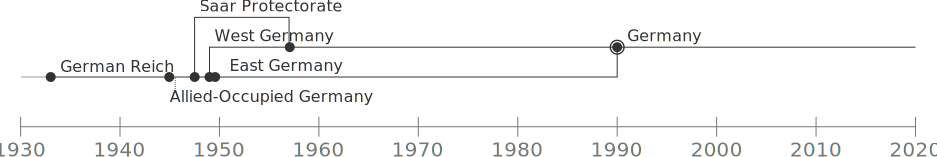
\includegraphics[width=0.9\textwidth]{graphics/development/hivent_model/histograph/example_germany}
  \caption{The concept of the HistoGraph at the example of Germany's history since 1945}
  \label{fig:example_germany}
\end{figure}


\begin{table}[ht]
\begin{center}
\begin{tabular}{l p{8.8cm} l}
  \toprule
  Hivent date & Hivent description & Hivent operations \\
  \midrule

    05.06.1945
  & \normalsize{In the Berlin Declaration the total dissolution of the Third Reich is confirmed. It separates into multiple parts, returning the territories annexed by the German Reich in World War II. The rest is controlled by the British, French, American and Soviet occupation zone.}
  & \texttt{SEP} \\[1.5em]

    16.02.1946
  & \normalsize{The Saar Protectorate is entangled from the French Zone of Occupation Germany, creating an own country.}
  & \texttt{SEC} \\[1.5em]

    28.05.1949
  & \normalsize{The Federal Republic of Germany (West Germany) is created from the British, American and French Zone of Occupation.}
  & \texttt{UNI} \\[1.5em]

    07.10.1949
  & \normalsize{The German Democratic Republic (East Germany) is created from the Soviet Zone of Occupation.}
  & \texttt{UNI} \\[1.5em]

    01.01.1957
  & \normalsize{The Saar Treaty (``Little Reunification'') joins the Saar Protectorate as the federal state ``Saarland'' in West Germany.}
  & \texttt{INC} \\[1.5em]

    03.10.1990
  & \normalsize{In the German Reunification, East joins West Germany. The Federal Republic of Germany is now called ``Germany''.}
  & \texttt{INC + NCH} \\[1.5em]

  \bottomrule
\end{tabular}
\caption{Historical events in German state history since 1945}
\label{tab:german_history_since_1945}
\end{center}
\end{table}

This example hosts a special case: In October 1949, East Germany was created from the Soviet Zone of Occupation. Both Areas have the same territory, but a different short and formal name. A \texttt{NCH} cannot be performed, because the identity is not preserved: the German Democratic Republic is a new Area. However, the change can be described by a \texttt{UNI} of only one old Area (Soviet zone), creating a new Area (East Germany). This new Area occupies exactly the same territory as the old Area and becomes the only historical successor of the old Area.

The graph plots Germany first. Since it does not have any successors, the plot expands only one way, historically backwards: East Germany and the Saar Protectorate were incorporated into Germany, so they are plotted. They emerged from the four post-war occupation zones, which are visualized in the next step. Each of the four occupation zones originated themselves from the German Reich. However, the German Reich dissolved into many more Areas, e.g.\ the Memel territory. They are not included in the graph, because they are not predecessors of any Area that is a recursive predecessor of present-day Germany.

Many problems of the graph visualization are apparent in this example: Circles may overlap if many operations happen in a short period of time -- in this case between 1945 and 1949.
The name ``West Germany'' collides with the vertical line indicating the incorporation of the Saar Protectorate, which should also be avoided.
Additionally, the names of the Areas of the four post-war occupation zones cannot be shown in the graph, due to lack of space.
One more important aspect can be seen in the foundation of West Germany in 1949: A \texttt{UNI} operation unifies three old Areas to one new Area. This could be visualized symmetrically with a straight line from the midmost incoming Area line into the circle to the outgoing Area line of the new Area. However, this would give the wrong impression that this midmost Area had the same identity as the newly created Area. In general, the circle for \texttt{UNI} and \texttt{SEP} operations with an odd number of old respectively new Areas must be displaced off the center to emphasize that the identity has changed.
All these issues are beyond the scope of this thesis and subject to future work in the field of Information Visualization.

% subsection histograph (end)

% section hivent_model (end)
%!TEX root = ../masters_thesis.tex

\section{Editing Hivent Data} % (fold)
\label{sec:editing_hivent_data}

The previous section proposed the abstract Hivent Model, a set of Hivent operations and a visualization method. However, one purpose of the HGIS developed in this thesis is to add, alter and delete historical changes. This section presents the tools and methods to edit spatio-temporal data about the evolution of Areas in the Hivent Model. Whereas the Hivent Operations are well-defined and specific, user studies have shown that they are not well understood by humans to edit Areas. This thesis therefore introduces a different set of six \emph{Edit Operations} in section \ref{sub:edit_operations}. Afterwards, section \ref{sub:edit_workflow} shows a \emph{workflow} to perform an Edit Operation step by step. The Hivent Model needs to support editing historical changes in between other historical changes. The last section \ref{sub:retrospective_updates} explains the theoretical approach to \emph{retrospecitve updates} of spatio-temporal data in the Hivent Model.


% ------------------------------------------------------------------------------
\subsection{Edit Operations} % (fold)
\label{sub:edit_operations}

The Hivent Operations are valuable, because they can describe all possible changes in the evolution of Areas in time and space. They are really well understood from the system point of view and form the basis for the Hivent Model. However, one purpose of the HGIS developed in this thesis is to provide a well understood user interface to edit historical changes to Areas.

Throughout the development process, interviews with researchers in humanities at University of Virginia were conducted to understand their mental model about the task. It turned out that the Hivent Operations are not suitable to be used for human edit purposes, because of their low-level nature. One example is that the operations do not provide a straightforward way to create a new Area on previously unclaimed land. The same is true for changing the formal name of an Area. Therefore, this thesis introduces a second set of operations: five high-level \emph{Edit Operations} describe changes to countries on the map (see table \ref{tab:edit_operations}). They have proven to be understandable in several user studies.

\vspace{0.5em}
\begin{table}[H]
\begin{center}
\begin{tabular}{m{0.75cm} m{0.8cm} m{2.4cm} m{9.1cm}}
  \raisebox{-0.35\height}
  {
\includegraphics[width=0.72cm]{graphics/development/edit_operations/CRE}} &
  \texttt{CRE} & Create &
  a new Area with a new name and territory on the map. \\

  \raisebox{-0.35\height}
  {
\includegraphics[width=0.72cm]{graphics/development/edit_operations/MRG}} &
  \texttt{MRG} & Merge &
  two or more Areas to a new Area. The name has to be set manually, the territory is automatically unified. \\

  \raisebox{-0.35\height}
  {\includegraphics[width=0.72cm]{graphics/development/edit_operations/DIS}} &
  \texttt{DIS} & Dissolve &
  one Area into two or more new Areas, manually setting their new territory and name. \\

  \raisebox{-0.35\height}
  {
\includegraphics[width=0.72cm]{graphics/development/edit_operations/CHB}} &
  \texttt{CHB} & Change Borders &
  between two neighboring Areas by defining the territory that changes sides. \\

  \raisebox{-0.35\height}
  {\includegraphics[width=0.72cm]{graphics/development/edit_operations/REN}} &
  \texttt{REN} & Rename &
  an Area and set a new formal name, short name or both. \\

  \vspace{0.35em}
  \raisebox{-0.35\height}
  {
\includegraphics[width=0.72cm]{graphics/development/edit_operations/CES}} &
  \texttt{CES} & Cease &
  an Area by deleting it from the map, leaving unclaimed land. \\

\end{tabular}
\caption{The six Edit Operations}
\label{tab:edit_operations}
\end{center}
\end{table}


% paragraph error_correction (end)

% subsection edit_operations (end)

% ------------------------------------------------------------------------------
\subsection{Edit Workflow} % (fold)
\label{sub:edit_workflow}

An Edit Operation describes an historical change that can be understood and performed by a user of the HGIS. This section shows that each Edit Operation can be internally expressed by a set of Hivent Operations. Therefore the Edit Operations are an abstraction layer in the Hivent Model between the Hivent and the Hivent Operations. To create an Edit Operation, four steps in a workflow need to be performed:

\begin{compactenum}
  \item Select the Areas that will be changed in the Edit Operation.
  \item For each new Area resulting from the Edit Operation, create a territory.
  \item For each new Area create a name.
  \item Add the Edit Operation to an Hivent to inherit the time point.
\end{compactenum}

For each Edit Operation, the requirements for the steps are different. Not all operations need all steps, because some data can be processed automatically. Table \ref{tab:editoperations_in_worklow} presents an overview about the behaviour of the Edit Operations in the first three steps. The last step is necessary for all.

\begin{table}[H]
\begin{center}
\begin{tabular}{m{0.9cm} m{4.2cm} m{4.2cm} m{3.5cm}}
  \toprule

  &
  \emph{Select old Areas} &
  \emph{Create new territories} &
  \emph{Create new names} \\

  \midrule
  \texttt{CRE} &
  -- &
  create a territory of the new country &
  create a name for the new country \\

  \midrule
  \texttt{MRG} &
  select the countries to be merged &
  \pbox{4.4cm}{--\\
  \footnotesize{territories of selected countries are automatically unified}} &
  create a name for the new country
  \\

  \midrule
  \texttt{DIS} &
  select a country to be \mbox{dissolved} &
  create a territory for each new country &
  create a name for each new country \\

  \midrule
  \texttt{CHB} &
  select two neighboring countries to change their border &
  \pbox{4.4cm}{create the new border between both countries \\
  \footnotesize{the territory for both countries will be created automatically}}  &
  -- \\

  \midrule
  \texttt{REN} &
  select a country to rename it &
  -- &
  create a new name of the country \\

  \midrule
  \texttt{CES} &
  select a country to cease it &
  -- &
  -- \\

  \bottomrule
\end{tabular}
\caption{The requirements of each step for the Edit Operations}
\label{tab:editoperations_in_worklow}
\end{center}
\end{table}

% - - - - - - - - - - - - - - - - - - - - - - - - - - - - - - - - - - - - - - -

% wording:
% UNI of "[old]"  to    "new"
% INC of "[old]"  into  "pres"
% SEP of "old"    into  "[new]"
% SEC of "[new]"  from  "pres"
% NCH of "pres"

\vspace{-1.0em}

Depending on the input of the user in the steps for an Edit Operation, there are different possibilities to express it by a set of Hivent Operations. Each Hivent Operation transforms a set of old Areas into a set of new Areas and can update the name or territory of one specific Area. All possibilities are introduced in table \ref{tab:editoperations_to_hg_operations}. Hivent Operations are combined when they happen at the same time. In the example of the German Reunification, East Germany was incorporated into West Germany which at the same time changed its short name to ``Germany'' (\texttt{INC + NCH}).

\begin{center}
\begin{longtable}{m{1.2cm} m{0.95cm} m{0.95cm} m{0.95cm} m{6.0cm} m{2.3cm}}
  \toprule

  \pbox{1.2cm}{EditOp.\\(case)} &
  \pbox{0.95cm}{old\\Areas\\[-0.8em]} &
  \pbox{0.95cm}{update\\Areas\\[-0.8em]} &
  \pbox{0.95cm}{new\\Areas\\[-0.8em]} &
  expression by Hivent Operations \protect\footnotemark &
  visualization \\
  \midrule
  \endhead

  % TODO: introduce T as territory that is used like a temporary Area with exactly that territoy

  %%% CREATE %%

  \multirow{9}{*}{\texttt{CRE} (1)} &
  \multicolumn{4}{p{10cm}}{
    Area $B_1$ is created with territory $T$. The part of $T$ that is on previously unclaimed land ($T_\Omega$) is seceded as $B_1$ from $\Omega$.
    If $T_\Omega$ is empty, then $B_1$ is initialized with an empty territory.
    The rest of $T$ covers some Areas $A_p$ partially and some Areas $A_f$ fully.
    For each $A_p$, the covered territory $T_p$ is seceded and incorporated into $B_1$.
    Each $A_f$ is completely incorporated into $B_1$.
  } &
  \multirow{9}{*}{
    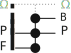
\includegraphics[width=2.5cm]{graphics/development/edit_to_hivent_operations/CRE_to_SEC+UNI}
  } \\

  &
  $n_f$ &
  $n_p$ &
  $1$ &
  \pbox{6.0cm}{
    ~\\
    \texttt{SEC} of $B_1$ from $\Omega$ \\
    \texttt{SEC} of $T_p$ from $A_p$, \texttt{INC} of $T_p$ into $B_1$ \\
    \texttt{INC} of $A_f$ into $B_1$
  } &
  \\

  %%% MERGE %%

  \midrule
  \multirow{3}{*}{\texttt{MRG} (1)} &
  \multicolumn{4}{p{10cm}}{
    Multiple Areas $A_i$ are unified to $B_1$. The new Area receives a name distinct from all the names of $A_i$.
  } &
  \multirow{3}{*}{
    
\includegraphics[width=2.5cm]{graphics/development/edit_to_hivent_operations/MRG_to_UNI}
  } \\
  &
  $n \geq 2$ &
  $0$ &
  $1$ &
  \pbox{6.0cm}{
    \texttt{UNI} of $\forall A_i$ to $B_1$
  } &
  \\

  \midrule
  \multirow{4}{*}{\texttt{MRG} (2)} &
  \multicolumn{4}{p{10cm}}{
    Multiple Areas $A_i$ are unified. The resulting Area reuses the short and formal name of one of the old Areas ($A_0$) and therefore preserves it. The remaining Areas $A_i$ are incorporated into $A_0$.
  } &
  \multirow{4}{*}{
    \includegraphics[width=2.5cm]{graphics/development/edit_to_hivent_operations/MRG_to_INC}
  } \\
  &
  $n \geq 1$ &
  $1$ &
  $1$ &
  \pbox{6.0cm}{
    \texttt{INC} of $\forall A_i$ into $A_0$
  } &
  \\

  \midrule
  \multirow{4}{*}{\texttt{MRG} (3)} &
  \multicolumn{4}{p{10cm}}{
    The same as the previous case, just that $A_0$ receives a new short name and therefore an additional name change is required.
  } &
  \multirow{4}{*}{
    \includegraphics[width=2.5cm]{graphics/development/edit_to_hivent_operations/MRG_to_INC+NCH}
  } \\
  &
  $n \geq 1$ &
  $1$ &
  $1$ &
  \pbox{6.0cm}{
    ~\\
    \texttt{INC} of $\forall A_i$ into $A_0$ \\
    \texttt{NCH} of $A_0$
  } &
  \\

  %%% DISSOLVE %%

  \midrule
  \multirow{4}{*}{\texttt{DIS} (1)} &
  \multicolumn{4}{p{10cm}}{
    Multiple Areas $B_i$ are separated from one initial Area $A_0$. Each $B_i$ receives a part of the territory of $A_0$ and a name. Each name is distinct from the name of $A_0$.
  } &
  \multirow{4}{*}{
    \includegraphics[width=2.5cm]{graphics/development/edit_to_hivent_operations/DIS_to_SEP}
  } \\
  &
  $1$ &
  $0$ &
  $n \geq 1$ &
  \pbox{6.0cm}{
    ~\\
    \texttt{SEP} of $A_1$ into $\forall B_i$
  } &
  \\

  \midrule
  \multirow{5}{*}{\texttt{DIS} (2)} &
  \multicolumn{4}{p{10cm}}{
    Multiple Areas $B_i$ are separated from one initial Area $A_0$. Each $B_i$ receives a part of the territory of $A_0$ and a name. One of the separated Areas has the same short and formal name as $A_0$, so it preserves its identity. The remaining new Areas secede from $A_0$.
  } &
  \multirow{5}{*}{
    \includegraphics[width=2.5cm]{graphics/development/edit_to_hivent_operations/DIS_to_SEC}
  } \\
  &
  $1$ &
  $1$ &
  $n \geq 1$ &
  \pbox{6.0cm}{
    ~\\
    \texttt{SEC} of $\forall B_i$ from $A_0$
  } &
  \\

  \midrule
  \multirow{4}{*}{\texttt{DIS} (3)} &
  \multicolumn{4}{p{10cm}}{
    The same as the previous case, just that $A_0$ receives a new short name and therefore an additional name change is required.
  } &
  \multirow{4}{*}{
    \includegraphics[width=2.5cm]{graphics/development/edit_to_hivent_operations/DIS_to_SEC+NCH}
  } \\
  &
  $1$ &
  $1$ &
  $n \geq 1$ &
  \pbox{6.0cm}{
    ~\\
    \texttt{SEC} of $\forall B_i$ from $A_0$  \\
    \texttt{NCH} of $A_p$
  } &
  \\

  %%% CHANGE BORDER %%%

  \midrule
  \multirow{10}{*}{\texttt{CHB} (1)} &
  \multicolumn{4}{p{10cm}}{
    One existing Area $A_0$ is selected and its territory changes. Relative to the old territory some parts of the territory expands ($T_e$) and some withdraws ($T_w$).
    The part of $T_e$ that expands into unclaimed land ($T_\Omega: T_\Omega \in T_e$) is seceded from $\Omega$ and incorporated into $A_0$.
    The Areas $A_f$ fully covered by $T_e$ are incorporated into $A_0$,
    the Areas $A_p$ partially covered by $T_e$ secede this territory $T_p \in T_e$ to $A_0$.
    $T_w$ is be incorporated into $\Omega$, resulting in unclaimed land.
  } &
  \multirow{10}{*}{
    \includegraphics[width=2.5cm]{graphics/development/edit_to_hivent_operations/CHB_to_SEC+INC_omega}
  } \\
  &
  $n_f$ &
  $1+n_p$ &
  $0$ &
  \pbox{6.0cm}{
    ~\\
    \texttt{SEC} of $T_\Omega$ from $\Omega$,
    \texttt{INC} of $T_\Omega$ into $A_0$ \\
    \texttt{SEC} of $T_p$ from $A_p$,
    \texttt{INC} of $T_p$ into $B_1$ \\
    \texttt{INC} of $A_f$ into $B_1$ \\
    \texttt{SEC} of $T_w$ from $B_1$,
    \texttt{INC} of $T_w$ into $\Omega$
  } &
  \\

  \midrule
  \multirow{7}{*}{\texttt{CHB} (2)} &
  \multicolumn{4}{p{10cm}}{
    Two existing Areas $A_1$ and $A_2$ are selected and their common border changes. This results in a symmetrical change of territories, made up by two sets of territories: $T_2$ that previously belonged to $A_1$ and is now part of $A_2$ and $T_1$ for which the opposite is true. $T_2$ is seceded by $A_1$ and incorporated into $A_2$, the opposite happenes to $T_1$.
  } &
  \multirow{7}{*}{
    \includegraphics[width=2.5cm]{graphics/development/edit_to_hivent_operations/CHB_to_SEC+INC}
  } \\
  &
  $0$ &
  $2$ &
  $0$ &
  \pbox{6.0cm}{
    ~\\
    \texttt{SEC} of $T_2$ from $A_1$,
    \texttt{INC} of $T_2$ into $A_2$ \\
    \texttt{SEC} of $T_1$ from $A_2$,
    \texttt{INC} of $T_1$ into $A_1$
  } &
  \\

  %%% RENAME %%%

  \midrule
  \multirow{3}{*}{\texttt{REN} (1)} &
  \multicolumn{4}{p{10cm}}{
    One Area $A_1$ is selected and both its short and formal name is changed. Therefore, a new Area $B_1$ is created as a direct successor of $A_1$. This is a special case of a unification with only one Area.
  } &
  \multirow{3}{*}{
    \includegraphics[width=2.5cm]{graphics/development/edit_to_hivent_operations/REN_to_UNI}
  } \\
  &
  $1$ &
  $0$ &
  $1$ &
  \pbox{6.0cm}{
    \texttt{UNI} of $A_1$ to $B_1$
  } &
  \\

  \midrule
  \multirow{3}{*}{\texttt{REN} (2)} &
  \multicolumn{4}{p{10cm}}{
    One Area $A_1$ is selected and receives a new short name, but the formal name and therefore the identity is preserved. $A_1$ is updated.
  } &
  \multirow{3}{*}{
    \includegraphics[width=2.5cm]{graphics/development/edit_to_hivent_operations/REN_to_NCH}
  } \\
  &
  $0$ &
  $1$ &
  $0$ &
  \pbox{6.0cm}{
    \texttt{NCH} of $A_1$
  } &
  \\

  %%% CEASE %%%

  \midrule
  \multirow{2}{*}{\texttt{CES} (1)} &
  \multicolumn{4}{p{10cm}}{
    One Area $A_1$ is selected and ceases by incorporating into the universe.
  } &
  \multirow{2}{*}{
    \includegraphics[width=2.5cm]{graphics/development/edit_to_hivent_operations/CES_to_INC}
  } \\
  &
  $1$ &
  $0$ &
  $0$ &
  \pbox{6.0cm}{
    \texttt{INC} of $A_1$ into $\Omega$
  } &
  \\

  \bottomrule
\caption{Translation from Edit Operations to Hivent Operations}
\end{longtable}
\label{tab:editoperations_to_hg_operations}
\end{center}
\footnotetext{multiple Hivent Operations in one row happen exactly at the same time point, so they are combined}


% subsection edit_workflow (end)

% ------------------------------------------------------------------------------
\subsection{Retrospective Updates} % (fold)
\label{sub:retrospective_updates}

A straighforward use case of the Hivent Model is to change the current state of the system with a new Edit Operation into the future. Givent the initial start point $t_0$, a current time point $t_{now} > t_0$ and a set of consecutively added Hivent Operations at $t_i \in [t_0 .. t_{now}[$. The accumulation of all changes make up the current state of the system at $t_{now}$. To change this current state, a new Hivent Operation can be inserted at $t_{now}$ into the future as a \emph{forward operation}. This state is valid until the next change is inserted.

For the purpose of historical research this use case alone is not sufficient, because the current state $t_{now}$ of the map is known to large degree. The problem is to edit states in the past. For this purpose the concept of a \emph{backward operation} comes into play: A Hivent Operation is inserted at time point $t_i$, but into the past: $ t_0 < t_i < t_{now}$. As an example: Given the initial state 10.06.2016 with present-day Germany created on 03.10.1990 on the map. The user wants to enter the German Reunification. The HGIS must support separating Germany into East and West, but indicating that this was the state \emph{before} 1990 and the original state was \emph{after} this date. This is complicated, because the conceptual, data and computational model have to adapt to this requirement.

The Hivent Operations themselves allow to be executed the other way, because each of them has an inverse operation: A \texttt{UNI} can be inverted with a \texttt{SEP} and a \texttt{INC} with a \texttt{SEC} operation. \texttt{NCH} can be inverted with itself by swapping the old and new name.

% - - - - - - - - - - - - - - - - - - - - - - - - - - - - - - - - - - - - - - -
\paragraph{Consistency} % (fold)
\label{par:consistency}

Each Hivent Operation that is not entered as a \emph{forward operation} to the end of the timeline must maintain the semantic, spatial and thematic integrity of the data, i.e. the changes to Areas, their territories and names must still work. All possible conflicts with consecutive Hivent Operations have to be resolved. The simple example in figure \ref{fig:update_conflict_example} shows the problem: Given time point $t_1$ with two Areas $A$ and $B$ and an \texttt{UNI} Hivent Operation at $t_2$ unifying $A$ and $B$ to $C$. If in retrospective a new Hivent Operation is inserted at $t_r: t_1 < t_r < t_2$ that cedes a part of of $A$ to a new Area $X$, the operation at $t_2$ is not consistent anymore, because the old territory of $A$ is not the same. It is not simple to say how the remaining territory $?$ should be treated.

\begin{figure}[H]
  \vspace{1em}
  \centering
  \includegraphics[width=0.8\textwidth]{graphics/development/update_conflict/example}
  \caption{Example for a simple conflict due to a retrospective update}
  \label{fig:update_conflict_example}
\end{figure}

% paragraph consistency (end)

% - - - - - - - - - - - - - - - - - - - - - - - - - - - - - - - - - - - - - - -
\paragraph{Conflicts} % (fold)
\label{par:conflicts}

The way the Hivent Model works is comparable to a version control system like \emph{Git}
\footnote{
  \emph{Git},
  --everything-is-local,
  \url{https://git-scm.com/},
  last access: 29.05.2016
}
Just like in Git, there are different kinds of conflicts that can occur on retrospective updates. In this model, they are classified regarding their resolvability:

\begin{compactenum}
  \item[A)] The conflict can be resolved \emph{\textbf{a}utomatically} without the interference of the user.
  \item[S)] The conflict requires the user to choose between two alternatives (\emph{\textbf{s}emi-automatic} resolution).
  \item[M)] The conflict is complex and the user needs to resolve it \emph{\textbf{m}anually}.
\end{compactenum}

The remaining part of this section examines all possible cases of conflicts and their resolveability. Each inserted Hivent Operation transforms a set of old Areas $A = [A_i]$ to a set of new Areas $B = [B_i]$ or updates an update Area $A_0$ or both. Each consecutive Hivent Operation that manipulates $A_0, A_i \in A$ or $B_i \in B$ has to be checked regarding three aspects of integrity:

\begin{compactenum}
  \item semantic: Does $A_0$ and $\forall A_i \in A$ still exist? If not, can it easily be replaced by another Area?
  \item spatial: Is the territory of $A_0$ and $\forall A_i \in A$ still the same? If not, can it easily by updated?
  \item thematic: Is the name of $A_0$ and $\forall A_i \in A$ still the same? If not, can it easily be updated?
\end{compactenum}

All cases can be broken down to the following scenario. Given an initial state at $t_1$ with three spatial entities on the map ($A_1, A_2, A_3$) and an Hivent Operation at $t_2$ manipulating this set of Areas with one of the five possible operations. This is operation is consistent and is called the original Hivent Operation ($H_o$). Now, a retrospective update $H_r$ with one of the five Hivent Operations manipulating the same set of Areas is inserted at $t_r: t_1 < t_r < t_2$. What happens regarding the semantic, spatial and thematic integrity of $H_o$? There are 25 possible cases, because there are 5 different $H_o$ and five different $H_r$ operations.

% paragraph conflicts (end)

% - - - - - - - - - - - - - - - - - - - - - - - - - - - - - - - - - - - - - - -
\paragraph{Retrospective Unification} % (fold)
\label{par:retrospective_unification}
\texttt{UNI}

% paragraph retrospective_unification (end)

% - - - - - - - - - - - - - - - - - - - - - - - - - - - - - - - - - - - - - - -
\paragraph{Retrospective Separation} % (fold)
\label{par:retrospective_separation}
\texttt{SEP}

% paragraph retrospective_separation (end)

% - - - - - - - - - - - - - - - - - - - - - - - - - - - - - - - - - - - - - - -
\paragraph{Retrospective Incorporation} % (fold)
\label{par:retrospective_incorporation}
\texttt{INC}

% paragraph retrospective_incorporation (end)

% - - - - - - - - - - - - - - - - - - - - - - - - - - - - - - - - - - - - - - -
\paragraph{Retrospective Secession} % (fold)
\label{par:retrospective_secession}
\texttt{SEC}

% paragraph retrospective_secession (end)

% - - - - - - - - - - - - - - - - - - - - - - - - - - - - - - - - - - - - - - -
\paragraph{Retrospective Name Change} % (fold)
\label{par:retrospective_name_change}
\texttt{NCH}

trallala und hoppsassa

% paragraph retrospective_name_change (end)

\vspace{1em}
The final result is visualized in the $5 \times 5$ matrix in figure \ref{tab:conflicts_retrospective_updates}.

\begin{table}[ht]
\begin{center}
\begin{tabular}{p{0.1cm} p{0.1cm} p{0.3cm} cx{2.0cm} cx{2.0cm} cx{2.0cm} cx{2.0cm} cx{2.0cm} cx{2.0cm}}
  \toprule
  & & & & \multicolumn{5}{c}{original Hivent Operation $H_o$} \\
  & & & & \texttt{UNI} & \texttt{SEP} & \texttt{INC} & \texttt{SEC} & \texttt{NCH} \\
  \midrule
    \multirow{5}{*}{\rot{retrospective}}
  & \multirow{5}{*}{\rot{operation $H_r$}}
    & & \texttt{UNI} & A & \textbf{M} & A & A & A \\
  & & & \texttt{SEP} & S(A$|$A) & S(A$|$A) & \textbf{M} & S(A$|$\textbf{M}) & A \\
  & & & \texttt{INC} & A & \textbf{M} & A & A & X \\
  & & & \texttt{SEC} & S(A$|$A) & S(A$|$A) & S(A$|$A) & S(A$|$A) & X \\
  & & & \texttt{NCH} & A & A & X & X & A \\
  \bottomrule
\end{tabular}
\caption{All possible conflicts on retrospective updates regarding their resolvability}
\small{X = no conflict, A = automatic, S = semi-automatic, \textbf{M} = manual resolution \\[-0.1em]
For semi-automatic resolution, the resolveability of the two options is stated like S(\nth{1}$|$\nth{2})}
\label{tab:conflicts_retrospective_updates}
\end{center}
\end{table}

% - - - - - - - - - - - - - - - - - - - - - - - - - - - - - - - - - - - - - - -
\paragraph{Error correction} % (fold)
\label{par:error_correction}

Correcting wrong information in an event-based system is important to understand: Given time point $t_y$ and an Area $A$ with the name $X$. If $X$ happens to be wrong, it means that the historical change at time point $t_x: t_x < t_y$ that created the name $X$ into Area $A$ is erroneous and has be corrected. Correcting a state means correcting the event that created this state.

% subsection retrospective_updates (end)

% section editing_hivent_data (end)
%!TEX root = ../masters_thesis.tex

\section{User Interface Design Process} % (fold)
\label{sec:user_interface_design_process}

The Hivent Model presented in the previous section serves as the data model for HistoGlobe, the application in which the work of this thesis is implemented. Developing the system bottom-up from the data model to the interface might not lead to usable system. Human Centered Design promotes a top-down process from the user via the interface into the core of the application. This section illustrates the iterative design process for this thesis seen in figure \ref{fig:hcd}. The two main use cases for HistoGlobe that are focused in this thesis are:

\begin{compactenum}
  \item \textbf{Understanding} the history of countries.
  \item \textbf{Editing} the spatio-temporal evolution of countries with historical changes.
\end{compactenum}

For both use cases a visualization and interaction was designed. The interviews with humanity researchers confirmed that the combination of a map and a timeline are a very appropriate and intuitive way to interactively visualize the history of countries. Thefore, the main concept of HistoGlobe introduced in section \ref{sec:histoglobe} does not need to be changed. However, two necessary extension modules have emerged: The \emph{HistoGraph} introduced in section \ref{sub:histograph} visualizes the history of countries on a graph. Next to the normal browsing mode, the \emph{Edit Mode} is proposed in section \ref{sub:edit_mode}. It uses the six Edit Operations to introduce historical changes to the current state on the map. The gradual process from the inital idea to the final user interface implemented in HistoGlobe is illustrated in the last section-

The user interface of HistoGlobe has two modi: The browsing mode to view the evolution of countries on a map with a timeline and the \emph{Edit Mode} to introduce historical changes to Areas. This mode is proposed in this section. The Human Centered Design process produced an interface that allows to intuitively edit Hivents, Areas and historical changes directly in HistoGlobe, without the need to write data into tables or forms.

The previous sections introduced the concepts of the HistoGraph and the Edit Mode. This section illustrates the Human Centered Design process integrating both concepts into the existing user interface of HistoGlobe. In each phase, interviews with students and employees of Scholar's Lab at University of Virginia were conducted to determine what works well and what has to be improved.

% - - - - - - - - - - - - - - - - - - - - - - - - - - - - - - - - - - - - - - -
\subsection{Initial interviews} % (fold)
\label{sub:initial_interviews}

The first phase, four researchers were asked about their opinions on the idea of HistoGlobe, potential use cases and the concept of the Edit Mode. The idea proved popular, especially for students and teachers in school, historically interested people in general and also for scholars in digital humanities. All researchers agreed that the key to successful Edit Mode is usability, because editing data in time and space is a challenging task. A main concern is uncertainty in historical research: Almost all sorts of information -- temporal, spatial and attribute -- are potentially uncertain. A good user interface for researchers therefore has to support uploading historical sources and indicating uncertainty. The Edit Operations from section \ref{sub:edit_operations} resulted from the initial interviews.

% subsection initial_interviews (end)


% - - - - - - - - - - - - - - - - - - - - - - - - - - - - - - - - - - - - - - -
\subsection{Paper Prototype} % (fold)
\label{sub:paper_prototype}

From the results of the inital interview, the first interface concept for the Edit Mode was developed and transformed into a paper prototype. It is an interface out of paper that is very fast to create and allows to identify flaws in the concept early in the design process. In this process, two paper prototype iterations were created. Both iteration took about three full work days: one day to create the conceptualize and create prototype, half a day to conduct the study with three people, and one and a half days to analyze the results and rethink the concept.

\begin{figure}[H]
\centering
\begin{subfigure}{.5\textwidth}
  \centering
  \includegraphics[width=225px]{graphics/development/design_process/paper_prototype_1.png}
\end{subfigure}%
\begin{subfigure}{.5\textwidth}
  \centering
  \includegraphics[width=225px]{graphics/development/design_process/paper_prototype_2.png}
\end{subfigure}
\caption{The two iteration of the paper prototype for the Edit Mode}
\label{fig:paper_prototypes}
\end{figure}

The interface consists of a map of Europe, a timeline centered at 1975 and the buttons with a set of dialogs for the for the Edit Mode. Both prototypes were evaluated with three test subjects that had to solve four tasks covering different use cases and operations:
\begin{compactenum}
  \item 1300: Rename incorrectly spelled name of Switzerland on the map (\emph{correction})
  \item 1990: Unite East and West Germany (\emph{forward change})
  \item 1993: Separate the Soviet Union into Russia, Estonia, Latvia, etc. (\emph{forward change})
  \item 1944: Change the border between Finland and the Soviet Union before 1944 (\emph{backward change})
\end{compactenum}

Most parts of the interface concept were understood and all subjects could solve the first three tasks. However, there were also problems:

\begin{compactenum}
  \item There difference between Hivents, the history of a country and an historical change was unclear.
  \item The border drawing dialoge was imagined to be very complex.
  \item The backward change was not understood
  \item Correcting the name Switzerland by changing the event that created it in 1300 caused confusion.
\end{compactenum}

The main finding of this step was that depending on the task, there is both an Hivent-based and an Area-based mental model of the task. This became apparent in the German Reunification Hivent: Some users started the unification operation first, and added West and East Germany afterwards -- and some selected first West Germany, then initiated a unification operation and then added East Germany. From that finding arose that the interface has to support both an Hivent-based and an Area-based approach to introduce historical changes and correct information on the map.

% subsection paper_prototype (end)

% - - - - - - - - - - - - - - - - - - - - - - - - - - - - - - - - - - - - - - -
\subsection{Mockup Prototype} % (fold)
\label{sub:mockup_prototype}

The main part of the design process was spent on the mockup prototypes. Their purpose is to rapidly develop an interface workflow that is understandable by the users. The prototypes were created in \emph{LibreOffice Impress}, an open-source slide-based presentation tool. The interface is simulated on slides: the map is a background image, the timeline, the set of buttons and dialogs for the Edit Mode and HistoGraph are modelled with geometric elements: lines, circles and rectangles. Interactivity is simulated by linking a click on an element to a different slide that shows the effect of the operation. This allows to model sudden changes in the interface.

\begin{figure}[ht]
  \centering
  \begin{subfigure}[b]{.5\textwidth}
    \centering
    \includegraphics[width=180px]{graphics/development/design_process/mockup_prototype_1.png}
  \end{subfigure}%
  \begin{subfigure}[b]{.5\textwidth}
    \centering
    \includegraphics[width=180px]{graphics/development/design_process/mockup_prototype_3.png}
  \end{subfigure} \\[0.8em]

  % \begin{subfigure}[b]{1.0\textwidth}
  %   \centering
  %   \includegraphics[width=325px]{graphics/development/design_process/mockup_prototype_3.png}
  % \end{subfigure}
  \caption{Two iteration stages of the mockup prototype for the Edit Mode}
  \label{fig:mockup_prototypes}
\end{figure}

Creating the mockup prototype took longer than a paper prototype, but would have still been much faster than actually implementing an interactive Web-based interface. Each prototype iteration was tested with multiple subjects and similar tasks as for the paper prototype. From one test to the next one changes to the interfaces were made. Some interesting quotes from the users were:

\begin{quoteit}
  \begin{tabular}{l r}
    ``this was much easier than I thought'' ~~~~~~~~ &
    ``there is a training session needed'' \\[0.5em]
    ``the interface is very clear &
    ``the logic makes sense, \\
    and graphically pleasing'' &
    it is just very complex'' \\[0.5em]
    ``it's looking good'' &
    ``a nice tutorial and a good \\
    & documentation are necessary'' \\
  \end{tabular}
\end{quoteit}

The main evolution was from a separate dialogue window for the Edit Operation workflow to an intergrated workflow window in the title bar. Also the HistoGraph was introduced to visualize the historical change at while editing it. A lot of smaller design issues, e.g. position of buttons, font sizes or color schemes were identified and fixed. But also conceptual issues arose.

Especially the problem to initiate a backward change (see section \ref{fig:backward_change}) proved to be very difficult. Two design solutions were developed: First, instead of initializing a change in 1990 to separate Germany into East and West, the user can introduce two creation events for the two German states in May and October 1949. The interface needs to provide a visual clue that after creating West Germany, this Area can only be active until 1990, because then another Area, present-day Germany, uses its territory (see figure \ref{sfig:backward_change_1}). The change from West Germany to Germany will be created automatically. The second approach is to introduce a button that flippes an Edit Operation that has just been created (see figure \ref{sfig:backward_change_2}) -- in this case the \texttt{DIS} operation introduced to secede East Germany from Germany will be flipped into a \texttt{UNI} operation to incorporate East Germany into Germany. This approach makes use of the fact that each Edit Operation and has an inverse, as explained in section \ref{par:inverse_operations}.
However, this flipping requires the introduction of additional creation events: West and East Germany were introduced in the change, but only the event that ceases both of them (\texttt{INC} of West Germany into East Germany). They also need a creation event, otherwise they would be active backwards all the way to $t_0$, the initial state of the system.

\begin{figure}[ht]
\centering
\begin{subfigure}[b]{.5\textwidth}
  \centering
  \includegraphics[width=200px]{graphics/development/design_process/backward_change_1.png}
  \caption{Visual clue: predefined and of Area}
  \label{sfig:backward_change_1}
\end{subfigure}%
\begin{subfigure}[b]{.5\textwidth}
  \centering
  \includegraphics[width=200px]{graphics/development/design_process/backward_change_2.png}
  \caption{Create backward change by flipping Edit Operation}
  \label{sfig:backward_change_2}
\end{subfigure}
\caption{Two approaches for editing changes backwards}
\label{fig:backward_change}
\end{figure}

The prototype was very valuable for the development process. In a total of two weeks, an interface concept and workflow was designed that proved to be understandable by the users.


% subsection mockup_prototype (end)

% - - - - - - - - - - - - - - - - - - - - - - - - - - - - - - - - - - - - - - -
\subsection{Web-based prototype} % (fold)
\label{sub:web_based_prototype}

The main advantage of the design process is that it prevents major redesigns of the final Web-based prototype. After three months of implementation of the final system, the interface looks very similar to the last version of the mockup prototype. The original main elements of the interface are the map, the timeline with the Now Marker indicating the current date of the visualization and the control buttons for zooming the map and the timeline. They are preserved and extended by new interface elements for the Edit Mode. Their interaction and behavior are introduced in this section at the example of the fictional secession of Scotland from the United Kingdom in 2018. The HistoGraph was not implemented, because of the conceptual problems mentioned in section \ref{sub:histograph} that have to be solved first.

\newpage
\begin{minipage}[t]{0.47\textwidth}

  \begin{figure}[H]
    \centering
    \includegraphics[width=1.0\textwidth]{graphics/development/final_interface/1_init.png}
    \caption{Initial state of the normal mode}
    \label{fig:final_1_init}
  \end{figure}

  The initial state of the user interface. Additional to the original elements, there is an edit button on the upper right corner. Clicking it enters the Edit Mode of the system.

\end{minipage}    % N.B. the % is very important
\hspace{1.5em}    % N.B. this must go in this line, no blank lines !!!
\begin{minipage}[t]{0.47\textwidth}

  \begin{figure}[H]
    \centering
    \includegraphics[width=1.0\textwidth]{graphics/development/final_interface/2_edit_mode.png}
    \caption{Initial state of the Edit Mode}
    \label{fig:final_2_edit_mode}
  \end{figure}

  In the Edit Mode, a title bar and six buttons for the Edit Operations are   revealed. Clicking a button starts the operation workflow introduced in section \ref{par:workflow}.

\end{minipage}

\vspace{1em}
\begin{minipage}[t]{0.47\textwidth}

  \begin{figure}[H]
    \centering
    \includegraphics[width=1.0\textwidth]{graphics/development/final_interface/3_select_old_areas.png}
    \caption{Step 1) \texttt{SELECT\_OLD\_AREAS}}
    \label{fig:final_3_select_old_areas}
  \end{figure}

  A \emph{Workflow Window} is guiding the user through the process of completing the historical change. It shows all the steps necessary for this Edit Operation. In the case of \texttt{DIS}, the user has to select the country to be dissolved by clicking it on the map. After the step is completed, clicking the next button in the workflow window procceeds to the next step. At each point in the workflow, clicking the back button reverts the previous action.

\end{minipage}    % N.B. the % is very important
\hspace{1.5em}    % N.B. this must go in this line, no blank lines !!!
\begin{minipage}[t]{0.47\textwidth}

  \begin{figure}[H]
    \centering
    \includegraphics[width=1.0\textwidth]{graphics/development/final_interface/4_set_new_territories.png}
    \caption{step 2) \texttt{SET\_NEW\_TERRITORIES}}
    \label{fig:final_4_set_new_territories}
  \end{figure}

  In the second step, the user has to create the territory for each new Area that shall be created. Therefore, the \emph{New Territory Tool} provides the functionality to create, manipulate and delete polylines by clicking and moving it directly on the map. The polypolygon drawn by the user is intersected with the old territory to create the territory of the new Area. After one new territory is created sucessfully, the second one can be taken from the remaining old territory by selecting it from the map. As soon as the whole old territory is distributed among the new Areas, the workflow proceeds to the next step.

\end{minipage}

\vspace{1em}
\begin{minipage}[t]{0.47\textwidth}

  \begin{figure}[H]
    \centering
    \includegraphics[width=1.0\textwidth]{graphics/development/final_interface/5_set_new_name.png}
    \caption{Step 3) \texttt{SET\_NEW\_NAMES}}
    \label{fig:final_5_set_new_name}
  \end{figure}

  In the next step, for each Area that has been created in the step before, a name has to be defined. The \emph{New Name Tool} is a draggable input form with two lines, the upper one for the short name, the lower one for the formal name, the identity of the Area. Via instant search, the user can select existing country names from the database to be put in the New Name Tool. When clicking the confirm button, the short name is put directly on the map.

\end{minipage}    % N.B. the % is very important
\hspace{1.5em}    % N.B. this must go in this line, no blank lines !!!
\begin{minipage}[t]{0.47\textwidth}

  \begin{figure}[H]
    \centering
    \includegraphics[width=1.0\textwidth]{graphics/development/final_interface/6_add_change_to_hivent_1.png}
    \caption{Step 4) \texttt{ADD\_CHANGE}}
    \label{fig:final_6_add_change_to_hivent_1}
  \end{figure}

  When all names are set, the Edit Operation is complete. In the last step of the workflow, it has to be added to an Hivent. The \emph{New Hivent Box} offers two possibilities: the user can search for an existing Hivent and add the historical change to it, or create a new one.

\end{minipage}

\vspace{1em}
\begin{minipage}[t]{0.47\textwidth}

  \begin{figure}[H]
    \centering
    \includegraphics[width=1.0\textwidth]{graphics/development/final_interface/7_add_change_to_hivent_2.png}
    \caption{Step 4) \texttt{ADD\_CHANGE}}
    \label{fig:final_7_add_change_to_hivent_2}
  \end{figure}

  The new Hivent created for that change is the ``Scottish Independence'' on 01.01.2018 with a description of the Hivent and possibly a location and a link to a wikipedia article. In the last line, the historical change ``Secession of Scotland from the United Kingdom'' is noted. Clicking the confirm button finalizes the workflow.

\end{minipage}    % N.B. the % is very important
\hspace{1.5em}    % N.B. this must go in this line, no blank lines !!!
\begin{minipage}[t]{0.47\textwidth}

  \begin{figure}[H]
    \centering
    \includegraphics[width=1.0\textwidth]{graphics/development/final_interface/8_final_state.png}
    \caption{The final state with Scotland}
    \label{fig:final_8_final_state}
  \end{figure}

  Clicking the edit button again leaves the Edit mode back to the normal view. Scotland and the United Kingdom are both visible on the map after 2018. When moving the timeline before 2018, Scotland is still part of the UK.

\end{minipage}

% subsection web_based_prototype (end)

% section user_interface_design_process (end)
%!TEX root = ../masters_thesis.tex

\section{Application} % (fold)
\label{sec:application}

HistoGlobe is a Web-based Historical Geographic Information System. The Data model and the conceptual model of the user interface were introduced in the first sections of this chapter. This section introduces the underlying database model, a specific implementation of the data model, and the computational model that translates between the conceptual model and the database model. The first part provides an overview about the architecture of the system in section \ref{sub:system_architecture}.
% ... bla bla bla, the rest comes last
% problems
% - support uncertainty

% ------------------------------------------------------------------------------
\subsection{System Architecture} % (fold)
\label{sub:system_architecture}

HistoGlobe uses a classical client-server architecture of a Web-based information system. The user opens the application and interacts with it through the user interface in a Web browser, the \emph{client} side of the system. The Web \emph{server} is a remote computer that hosts the database and the middleware. The user interacts with the interface and the client-side application sends a request to the Web server for new data. The middleware checks the request and queries the necessary data from the database. It transforms the data and sends it back to the client. The interface shows the new information.

\begin{figure}[H]
  \vspace{1em}
  \centering
  \includegraphics[width=0.7\textwidth]{graphics/development/system_architecture}
  \caption{The system architecture of HistoGlobe}
  \label{fig:system_architecture}
\end{figure}

This clear separation between the data, the application and the user interaction in this chapter and in the system follows directly from the \emph{model-view-controller} pattern: One part can be changed independently from the others parts: if the 2D map is replaced by a 3D globe, only the view changes, but the middleware and the database can stay untouched. Likewise, the implementation of a new database technology has no consequences to the view.

% subsection system_architecture (end)

% ------------------------------------------------------------------------------
\subsection{Hivent Database Model} % (fold)
\label{sub:database_model}

The underlying Hivent Model is implemented in the spatio-temporal \emph{Hivent Database Model}. HistoGlobe uses \emph{Django}, a free and open-source web framework
\footnote{
  \emph{Django},
  The Web framework for perfectionists with deadlines,
  URL: \url{https://www.djangoproject.com/},
  last access: 27.05.2016
},
combined with \emph{PostgreSQL}
\footnote{
  \emph{PostgreSQL:},
  The world's most advanced open source database,
  URL: \url{http://www.postgresql.org/},
  last access: 31.10.2015
}
, one of the most popular Object-Relational Database Management Systems introduced in section \ref{sub:object_relational_database_management_systems}, on the server-side of the system. This allows HistoGlobe to take advantage of object-oriented concepts in a stable and fast relational database. Since the database is using a lot of geospatial data, \emph{PostGIS} is used as a spatial database extension for PostgreSQL
\footnote{
  \emph{PostGIS},
  Spatial and Geographic Objects for PostgreSQL,
  URL: \url{http://postgis.net/},
  last access: 27.05.2016
}.

With these tools at hand, the database model shown in figure \ref{fig:database_model_er} was developed. It is the final result of a highly iterative process that underwent many improvements and adpations to new requirements introduced in the Human Centered Design process. The model is structured in two parts covereing four different domains of the spatio-temporal model: The lower part describes the semantic, spatial and thematic domain of Areas and the upper part represents the temporal domain of Hivents that introduces changes to the Areas.

\begin{figure}[ht]
  \centering
  \includegraphics[width=0.8\textwidth]{graphics/development/database_model/er_model}
  \caption{The Hivent Database Model}
  \small{Each entity additionally has an \texttt{id} attribute, which is omitted for simplification purposes.}
  \label{fig:database_model_er}
\end{figure}

% - - - - - - - - - - - - - - - - - - - - - - - - - - - - - - - - - - - - - - -
\paragraph{Semantic, Spatial and Thematic Domain} % (fold)
\label{par:semantic_spatial_and_thematic_domain}

In the Hivent Model, the entity visible on the map is an Area with a name and a territory, as introduced in section \ref{sec:hivent_model}. In the database model, they are represented by three entities:

\begin{enumerate}
  \item \texttt{Area}: semantic domain defining one identical Area with potentially changing name and territory. The \texttt{universe} attribute is true for $\Omega$, for the other Areas it is false.
  \item \texttt{AreaTerritory}: spatial domain. A polypolygon describes the \texttt{geometry} of the territory and a \texttt{representative\_point} the position of the name label on the map.
  \item \texttt{AreaName}: thematic domain. It is defined by a \texttt{short\_name} and a \texttt{formal\_name}.
\end{enumerate}

% paragraph semantic_spatial_and_thematic_domain (end)

% - - - - - - - - - - - - - - - - - - - - - - - - - - - - - - - - - - - - - - -
\paragraph{Temporal Domain} % (fold)
\label{par:temporal_domain}

The main idea of the model is that the Areas can change over time. These changes are introduced by \texttt{Hivents}, the main entitity of the eponymic model with five attributes: The \texttt{name} and a textual \texttt{description} of the Hivent, the point in time the Hvent happend (\texttt{date}), the Hivent \texttt{location} as a simple string and a \texttt{link} (URL) to the related article, serving as a historical source. Each Hivent can introduce a set of \texttt{EditOperation}s introduced and understood by the user. They consist themselves of a set of low-level \texttt{HiventOperation}s). They replace a set of \texttt{OldArea}s with a set of \texttt{NewArea}s and might update the name or the territory of one specific \texttt{UpdateArea}.

% paragraph temporal_domain (end)

% - - - - - - - - - - - - - - - - - - - - - - - - - - - - - - - - - - - - - - -
\paragraph{Example} % (fold)
\label{par:example}

Figure \ref{fig:database_example_reunification} shows the Hivent Database Model at the example of the German Reunification on 3. October 1990. Before 1990, there were the Areas \texttt{GDR} (``German Democratic Republic'', East Germany) and \texttt{FRG} (``Federal Republic of Germany'', West Germany). A user introduced a Merge operation (\texttt{MRG}) in the Edit Mode between \texttt{FRG} and \texttt{GDR}. The new Area received the short name ``Germany'' and the same formal name ``Federal Republic of Germany'' as previous West Germany. Internally, the Edit Mode translates this to an \texttt{INC} of \texttt{GBDR} into \texttt{FRG} and a subsequent \texttt{NCH} of the \texttt{FRG}. One Area ceases, one Area is updated twice and no new Area is created.

\begin{figure}[ht]
  \vspace{1em}
  \includegraphics[width=0.9\textwidth]{graphics/development/database_model/example_reunification}
  \caption{Visualization of the German Reunification in the Hivent Database Model}
  \label{fig:database_example_reunification}
\end{figure}


% paragraph example (end)

% - - - - - - - - - - - - - - - - - - - - - - - - - - - - - - - - - - - - - - -
\paragraph{Initial Dataset} % (fold)
\label{par:initial_dataset}

Section \ref{sub:data_sources} explained the lack of data about historical countries. It is out of the scope of this thesis to create a large testing dataset with the historical countries in the world. The inital dataset consists of the following countries, their names and borders: the 193 UN members and 2 observer states (created by \texttt{CRE} operation) and seven countries with limited international recognition: Kosovo, Transnistria, South Ossetia, Abkhazia, Nagorno-Karabakh, Somaliland and Sahrawi Arab Democratic Republic, see section \ref{par:un_non_members_with_limited_recognition}) (created by \texttt{DIS} operations from their homeland on the day of their declaration of independence).

% paragraph initial_dataset (end)

% - - - - - - - - - - - - - - - - - - - - - - - - - - - - - - - - - - - - - - -
\paragraph{Middleware} % (fold)
\label{par:middleware}

The Django web framework provides \emph{view} classes as the middleware that receives requests from the client, processes them, queries the necessary data from the database and returns an \texttt{HttpResponse} back to the client. In the naive implementation of the system, the middleware provides only two views for the two use cases:

\begin{enumerate}
  \item \textbf{\texttt{get\_all}} is initially called by the client side on loading the web service. The server responds to this \texttt{HttpRequest} with all data from the database in one \emph{JSON} object. While this behaviour is not scalable, for the initial dataset it was sufficient: The data was loaded in 3.5 seconds.
  \item \textbf{\texttt{save\_edit\_operation}} is called by the client after an Edit Operation has been completely created in the Edit Mode. In the last step, the client assembles the relevant data: the associated \texttt{Hivent} and \texttt{HiventOperation}s), data about each \texttt{OldArea}, \texttt{UpdateArea} and \texttt{NewArea}. The view checks the data for integrity and stores them in the database. The method returns to the client a confirmation and a set of final \texttt{id}s for the entities stored in the database.
\end{enumerate}

% paragraph middleware (end)

% subsection database_model (end)

% ------------------------------------------------------------------------------
\subsection{Classes} % (fold)
\label{sub:classes}

% HERE GOES IT WIDER %

Class diagram

HistoGlobe

SpatialDisplay -> Map

TimeController  <-> Timeline
                <-> NowMarker

HiventController                AreaController <->  AreasOnMap
HiventHandle                    AreaHandle
Hivent
HistoricalChange    AreaChange  Area
                                AreaName            AreaNameLayerOnMap
                                AreaTerritory       AreaTerritoryLayerOnMap

DatabaseInterface

EditMode -> EditOperation -> EditOperationStep
NewTerritoryTool* NewNameTool NewHiventBox
WorkflowWindow

HistoGraph

LabelManager*

important little utils
  Button, ButtonArea
  NumberInput, TextInput, TextInputArea
  Title
  Watermark
  DoublyLinkedList
  WithinTree
  Geometry -> Polypolygon -> Polygon -> Polyline -> Point


% subsection classes (end)

% section application (end)

% chapter development (end)

% ==============================================================================

\vspace{2em}
transition to next chapter
%!TEX root = ../masters_thesis.tex

\chapter{Evaluation} % (fold)
\label{cha:evaluation}

% The section closes with an informal proof that the model is approproate.


% chapter evaluation (end)

% ==============================================================================
\vspace{2em}

transition to extensions
\include{chapter/5-extension}
%!TEX root = ../masters_thesis.tex

\chapter{Summary} % (fold)
\label{cha:summary}


% ==============================================================================
\section{Results} % (fold)
\label{sec:results}

% section results (end)


\paragraph{Research Questions} % (fold)
\label{par:result_research_questions}

% paragraph result_research_questions (end)


% ==============================================================================
\section{Problems} % (fold)
\label{sec:problems}

% section problems (end)



% ==============================================================================
\section{Future Work} % (fold)
\label{sec:future_work}

step further: temporal GIS to narrative GIS

idea: explain history with spatial narratives
  geographically contextualize events and interactions
  organizing principle: time

extend the pure presentational purpose of st data to analytical purpose, e.g. where have most border changes take place in previous 200 years?

Another problem for historians is that they do not necessarily need a tool to better visualize existing knowledge (e.g. historical maps), but to generate new knowledge by analyzing spatio-temporal coherences or distributions in historical data. Spatio-temporal reasoning is still an open field and not easily possible with existing HGIS

\cite[p. 268]{knowles2008placing}, \cite[p. xii]{gregory2014toward}.
space-time premise by Gaddis 2002
  time and space equal importance
  event     what significantly has happend and by whom? (singularity!)
  process   how something has happened? (event+activity => trigger of process)
  change    driven by process
  spatiotemporal data defines all above three
  % \cite Gaddis 2002


% section future_work (end)


% ==============================================================================

% chapter summary (end)


%\* BIBLIOGRAPHY*\

% reduce font size of bibliography
{\footnotesize{
  \bibliography{chapter/sources}{}
}}
\bibliographystyle{chapter/alphaurl}


%\* APPENDIX *\

%!TEX root = ../thesis.tex

\section*{Stuff} % (fold)
\label{sec:stuff}

% section stuff (end)



\end{document}
